\chapter{Results}

\section{Calculation of bulk properties}

The current work is aimed to study the structure of OH defects in LiFePO$_4$ and LiMnPO$_4$.
However, first of all the calculation of the lattice constants and electric properties of pure material are necessary to benchmark the chosen calculation parameters. The  LiFePO$_4$ unit cell obtained after optimization of lattice constants and atomic positions in shown in  Figure~\ref{ris:uc}. The obtained lattice constants for LiFePO$_4$ and LiMnPO$_4$ are in good agreement with literature data, which is seen from  Table~\ref{table:uc}. 

\begin{figure}[ht]
\begin{minipage}[h]{0.9\linewidth}
\center{\includegraphics[width=1\linewidth]{pictures/LFP_uc.png}}
\end{minipage}
\caption{Schematic unit cell and features of LiFePO$_4$ and LiMnPO$_4$}
\label{ris:uc}
\end{figure}

\begin{table}[h]
\center{
\caption{Lattice constants and band gaps for LiFePO$_4$ and LiMnPO$_4$ in comparison to literature data }
\begin{tabular}{|c|c|c|c|c|}
    \cline{1-5}
    & \multicolumn{2}{|c|} {LiFePO$_4$} & \multicolumn{2}{|c|} {LiMnPO$_4$} \\
    \cline{1-5}
    Space group & \multicolumn{4}{|c|} {$Pnma$} \\
    \cline{1-5}
    & Current & Ref. & Current & Ref.  \\
    & work &  &  work &  \\
    \cline{2-5}
    & & & & \\
    $a,${~\AA} & 10.33 & 10.32 \cite{urusova2017magnetic} & 10.56 & 10.45 \cite{urusova2017magnetic} \\
    $b,${~\AA} & 6.01 & 6.01 \cite{urusova2017magnetic} & 6.15  & 6.10 \cite{urusova2017magnetic} \\
    $c,${~\AA} & 4.73  & 4.69 \cite{urusova2017magnetic} & 4.79  & 4.74 \cite{urusova2017magnetic} \\
    Band gap, eV & 0.0 (GGA) & 0.2 (GGA) & 2.1 (GGA) & 2.0 (GGA) \\
                 &  & 3.7 (+U) \cite{zaghib2007electronic} &  & 3.8 (+U) \cite{zaghib2007electronic} \\
    \cline{2-5}
    & \multicolumn{2}{|c|}{} & \multicolumn{2}{|c|}{} \\
    Voltage, V & \multicolumn{2}{|c|}{3.4 \cite{li2002limnpo4}}  & \multicolumn{2}{|c|}{4.1 \cite{li2002limnpo4}}  \\
    Capacity, mAh/g & \multicolumn{2}{|c|}{150 \cite{li2002limnpo4}} & \multicolumn{2}{|c|}{140 \cite{li2002limnpo4}} \\
    \cline{1-5} 
\end{tabular}
\label{table:uc}
}
\end{table}

The calculated total density of states (DOS) is shown in Figure~\ref{ris:bs} for LiFePO$_4$ and LiMnPO$_4$ compounds. 
In the case of LiMnPO$_4$ the obtained band gap is 2.1 eV, which agrees with insulating behaviour of this material, observed in experiment. However, the value of band gap is underestimated, which is a well known problem of GGA calculations for transition metal compounds, where localization of d-electrons results in band gap opening. 
In the case of LiFePO$_4$ our GGA calculations predict the absence of band gap. 
By using Hubbard correction, the localization of d-electrons is taken into account and the band gap can be reproduced in agreement to the experiment. While the Hubbard correction has significant influence on formation energies, the GGA without U can still be used for describing structural features of point defects as will be shown further.

\begin{figure}[h]
\begin{minipage}[h]{0.49\linewidth}
\center{\includegraphics[width=1.0\linewidth]{pictures/LFP_dos.png} \\ a) LiFePO$_4$ }
\end{minipage}
\hfill
\begin{minipage}[ht]{0.49\linewidth}
\center{\includegraphics[width=0.94\linewidth]{pictures/LMP_dos.png} \\ b) LiMnPO$_4$ }
\end{minipage}
\caption{Calculated total density of states with GGA approach for LiFePO$_4$ and LiMnPO$_4$ compounds.}
\label{ris:bs}
\end{figure}

\section{Structure and energetics of H interstitial and  Li/H and Fe/2H substitution defects}

In this section the formation energy of P vacancy and several OH defects are calculated with GGA and GGA+U methods. To compare interstitial H and substitutional Li/H and Fe/2H we use a simple thermodynamic model which takes into account the stability region LiFePO$_4$ phase. Though this model does not correspond directly to the synthesis conditions, which are too complicated for theortical reproductions, it gives reasonable estimation of defect formation energies and allows to compare them with each other. 
We begin from from Li-Fe-P-O phase diagram, which was constructed from first-principles by Ong et al. ~\cite{ong2008li}. The region of interest is formed by Li$_3$PO$_4$, LiFePO$_4$ and Fe$_2$O$_3$ end phases (Figure~\ref{ris:PhaseD}). The chemical potential, $\mu (X)$ of each species is then defined using end phases and the chemical potential of O$_2$. The latter is determined from the experiment conditions and changed from the temperature, pressure, and concentration of reductive chemical additions. According to Ong et al. the relevant values of oxygen chemical potential varies from --13.10 to --11.52 eV ~\cite{ong2008li}. The chemical potential of hydrogen is calculated with respect to water molecule in the gas phase according to the following equation~(\ref{eq:muH}):

\begin{equation}
    \mu(\rm H)=\frac{1}{2}[\mu(\rm H_2O_{gas})-\frac{1}{2}\mu(\rm O_2)]
\label{eq:muH}
\end{equation}

\begin{figure}[h]
\center{\includegraphics[width=0.6\linewidth]{pictures/Phase_diagram.png} \\ }
\caption{Phase diagram for LiFePO$_4$ compounds~\cite{ong2008li}}
\label{ris:PhaseD}
\end{figure}

The energy of H$_2$O in the gas phase is calculated from the first-principle study at 0~(K). The chemical potentials of Li, Fe, and P species are determined from the total energies of Li$_3$PO$_4$, LiFePO$_4$ and Fe$_2$O$_3$ phases according to the following equations:

\begin{eqnarray}
\label{FeLiP}
  &\mu(\rm Fe)=\frac{1}{2}[\mu(\rm Fe_2O_3)-\frac{3}{2}\mu(\rm O_2)] \nonumber \\ 
  &\mu(\rm Li)=\frac{1}{2}[\mu(\rm Li_3PO_4)-\mu(\rm LiFePO_4)+\mu(\rm Fe)] \\
  &\mu(\rm P)=\frac{1}{2}[3\mu(\rm LiFePO_4)-\mu(\rm Li_3PO_4)-3\cdot\mu(\rm Fe)-4\cdot\mu(\rm O_2)] \nonumber
\end{eqnarray}

At most oxidizing chemical potential of oxygen $\mu (O_2)$ = --11.52 eV, the chemical potentials of each species are  --4.650 eV for H, --5.821 eV for Li, --10.095 eV for Fe, and --10.048 eV for P.

According to the chemical potential values of each species the formation energies of Li, Fe or P vacancies in LiFePO$_4$ are calculated using the energies of Li$_{1-x}$Vac$_{x}$FePO$_4$,  LiFe$_{1-x}$Vac$_{x}$PO$_4$  and LiFeP$_{1-x}$Vac$_{x}$O$_4$ supercells, according to these equations:

\begin{eqnarray}
\label{eq:FeLiP1}
  &E(\rm Li_{vacancy})=E(\rm Li_{1-x}Vac_{x}FePO_4)-E(\rm LiFePO_4)+\mu(\rm Li) \nonumber \\ 
  &E(\rm Fe_{vacancy})=E(\rm LiFe_{1-x}Vac_{x}PO_4)-E(\rm LiFePO_4)+\mu(\rm Fe) \\
  &E(\rm P_{vacancy})=E(\rm LiFeP_{1-x}Vac_{x}O_4)-E(\rm LiFePO_4)+\mu(\rm P) \nonumber
\end{eqnarray}

The calculated formation energies are presented in Table~\ref{tabular:form_en}.

\begin{table}[h]
\caption{Chemical potentials of species and formation energies of  vacancies in LiFePO$_4$ ($\mu$ (O$_2$)=--11.52 eV) calculated with GGA and GGA+U methods}
\label{tabular:form_en}
\begin{center}
\begin{tabular}{|c|c|c|c|c|}
\hline
& & & & \\
\textbf{Type} & \textbf{$\mu (X)$, eV} & \textbf{$\mu (X)$, eV} & \textbf{E$_{vacancy}$, eV} & \textbf{E$_{vacancy}$, eV} \\
\textbf{of atom} & \textbf{(GGA)} & \textbf{(GGA+U)} & \textbf{(GGA)} & \textbf{(GGA+U)} \\
\hline
&  & & & \\
H & -- 4.650 & -- 4.650 & -- & -- \\ 
\hline
&  & & & \\
Li & -- 5.821 & -- 5.239 & -- 1.75 & 0.64\\ 
\hline
& & & & \\
Fe & -- 10.095 & -- 8.328 & -- 2.48 & 1.40 \\ 
\hline
& & & & \\
P & -- 10.048 & -- 11.626 & 0.38 & 3.46 \\ 
\hline
\end{tabular}
\end{center}
\end{table}

A comparison of chemical potentials obtained with GGA and GGA+U calculations shows the difference for the iron atom, which is expected, since the U correction is applied on its d orbitals. As a result such behaviour have significant impact on formation energies of vacancies. As it can be seen from Table~\ref{tabular:form_en}, the GGA without U considerably underestimates vacancy formation energies. 
This correlates well with the known underestimation of Li intercalation potentials and Li vacancy formation energies by GGA method in transition metal compounds.
Thus, the GGA+U calculation is more appropriate for a realistic estimate of energies, but, at the same time, the atomic structure can be reproduced with GGA.

\textbf{Interstitial hydrogen in  octahedral voids of ideal LiFePO$_4$}

We found two stable hydrogen positions in octahedral void of LiFePO$_4$ structure. 

In the first case the H atom was initially placed near the Fe atom with Fe-H distance of 1.95~{\AA}. After atomic optimization the Fe-H distance is 1.99~{\AA}, the shortest O-H distance is 1.04{~\AA}, and second shortest O-H distance is 1.55{~\AA}. The H atom is located at line between O1 and O2 atoms, creating the hydrogen bond, Figure~\ref{ris:oct1}. The formation energy of such defect is equal to 3.35 eV.

In the second case the hydrogen atom was placed near the P atom (Figure~\ref{ris:oct2} a)). After atomic  relaxation the distance between the H atom and O is 1.01{~\AA} and the distance between the hydrogen atom and the second neighboring oxygen H-O$_2$ is 1.84{~\AA}, Figure~\ref{ris:oct2}. The formation energy of such defect is slightly lower and is equal to 3.22~eV.


\begin{figure}[ht]
\begin{minipage}[ht]{0.49\linewidth}
\center{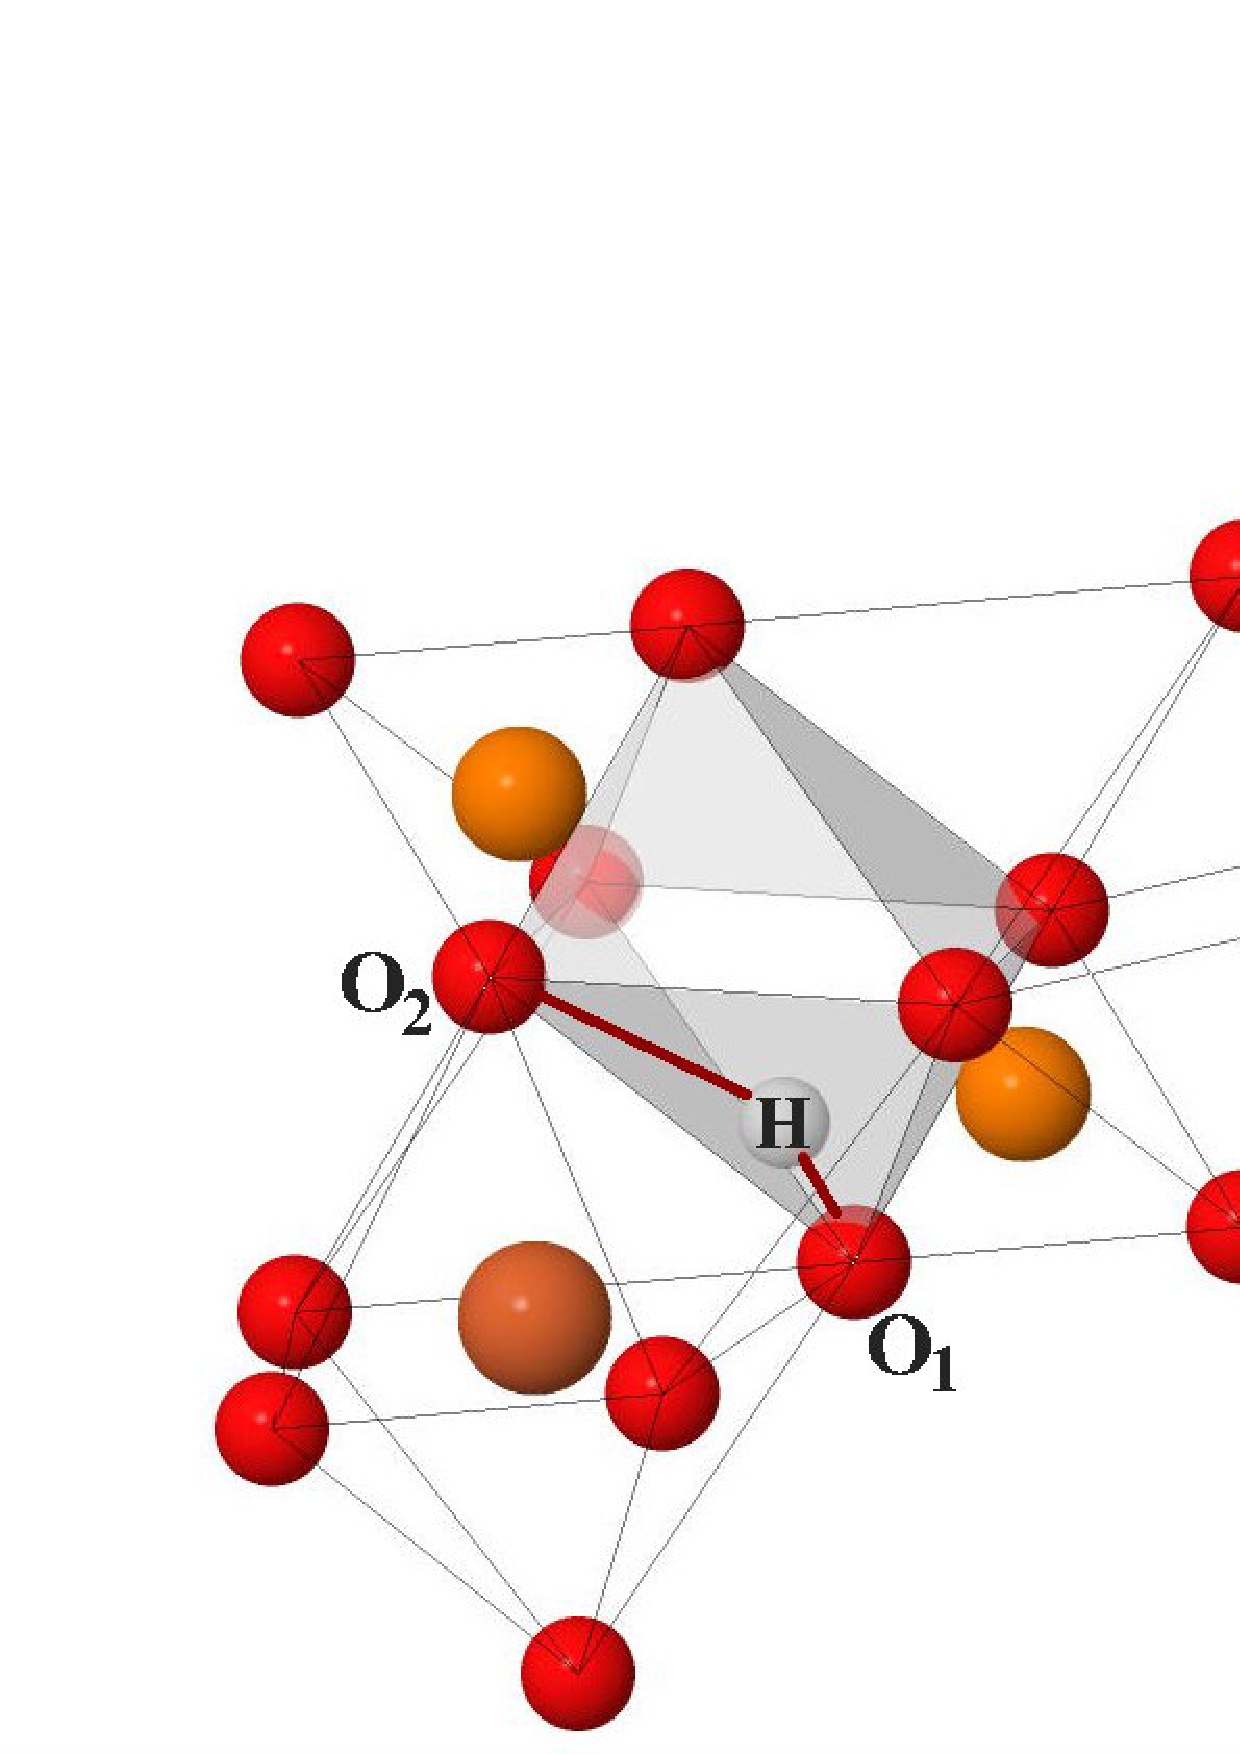
\includegraphics[width=0.9\linewidth]{pictures/oct1beforeCROP.png} \\ a)}
\end{minipage}
\hfill
\begin{minipage}[ht]{0.49\linewidth}
\center{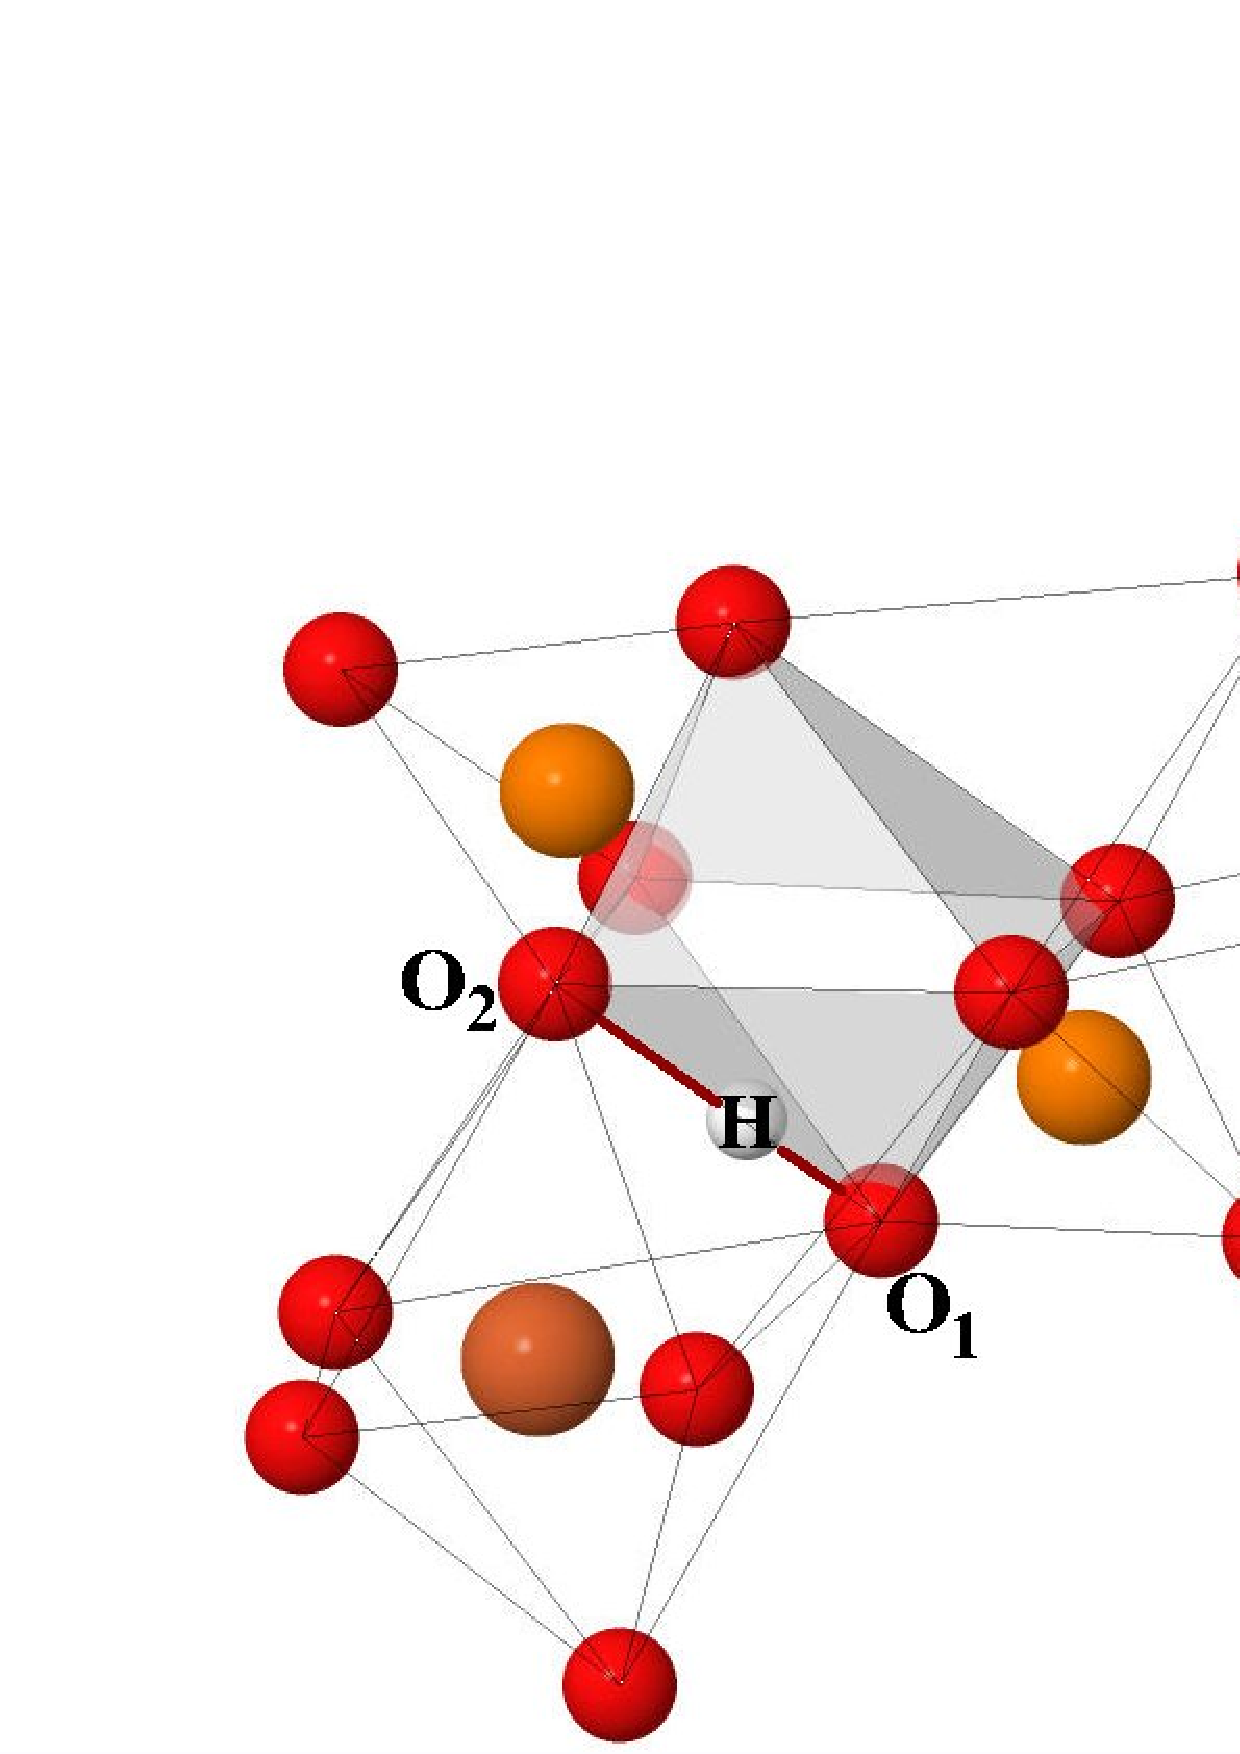
\includegraphics[width=0.9\linewidth]{pictures/oct1afterCROP.png} \\ b)}
\end{minipage}
\caption{Position of H atom in octahedral void before (a) and after (b) structural optimization (case 1)}
\label{ris:oct1}
\end{figure}

\begin{figure}[ht]
\begin{minipage}[h]{0.49\linewidth}
\center{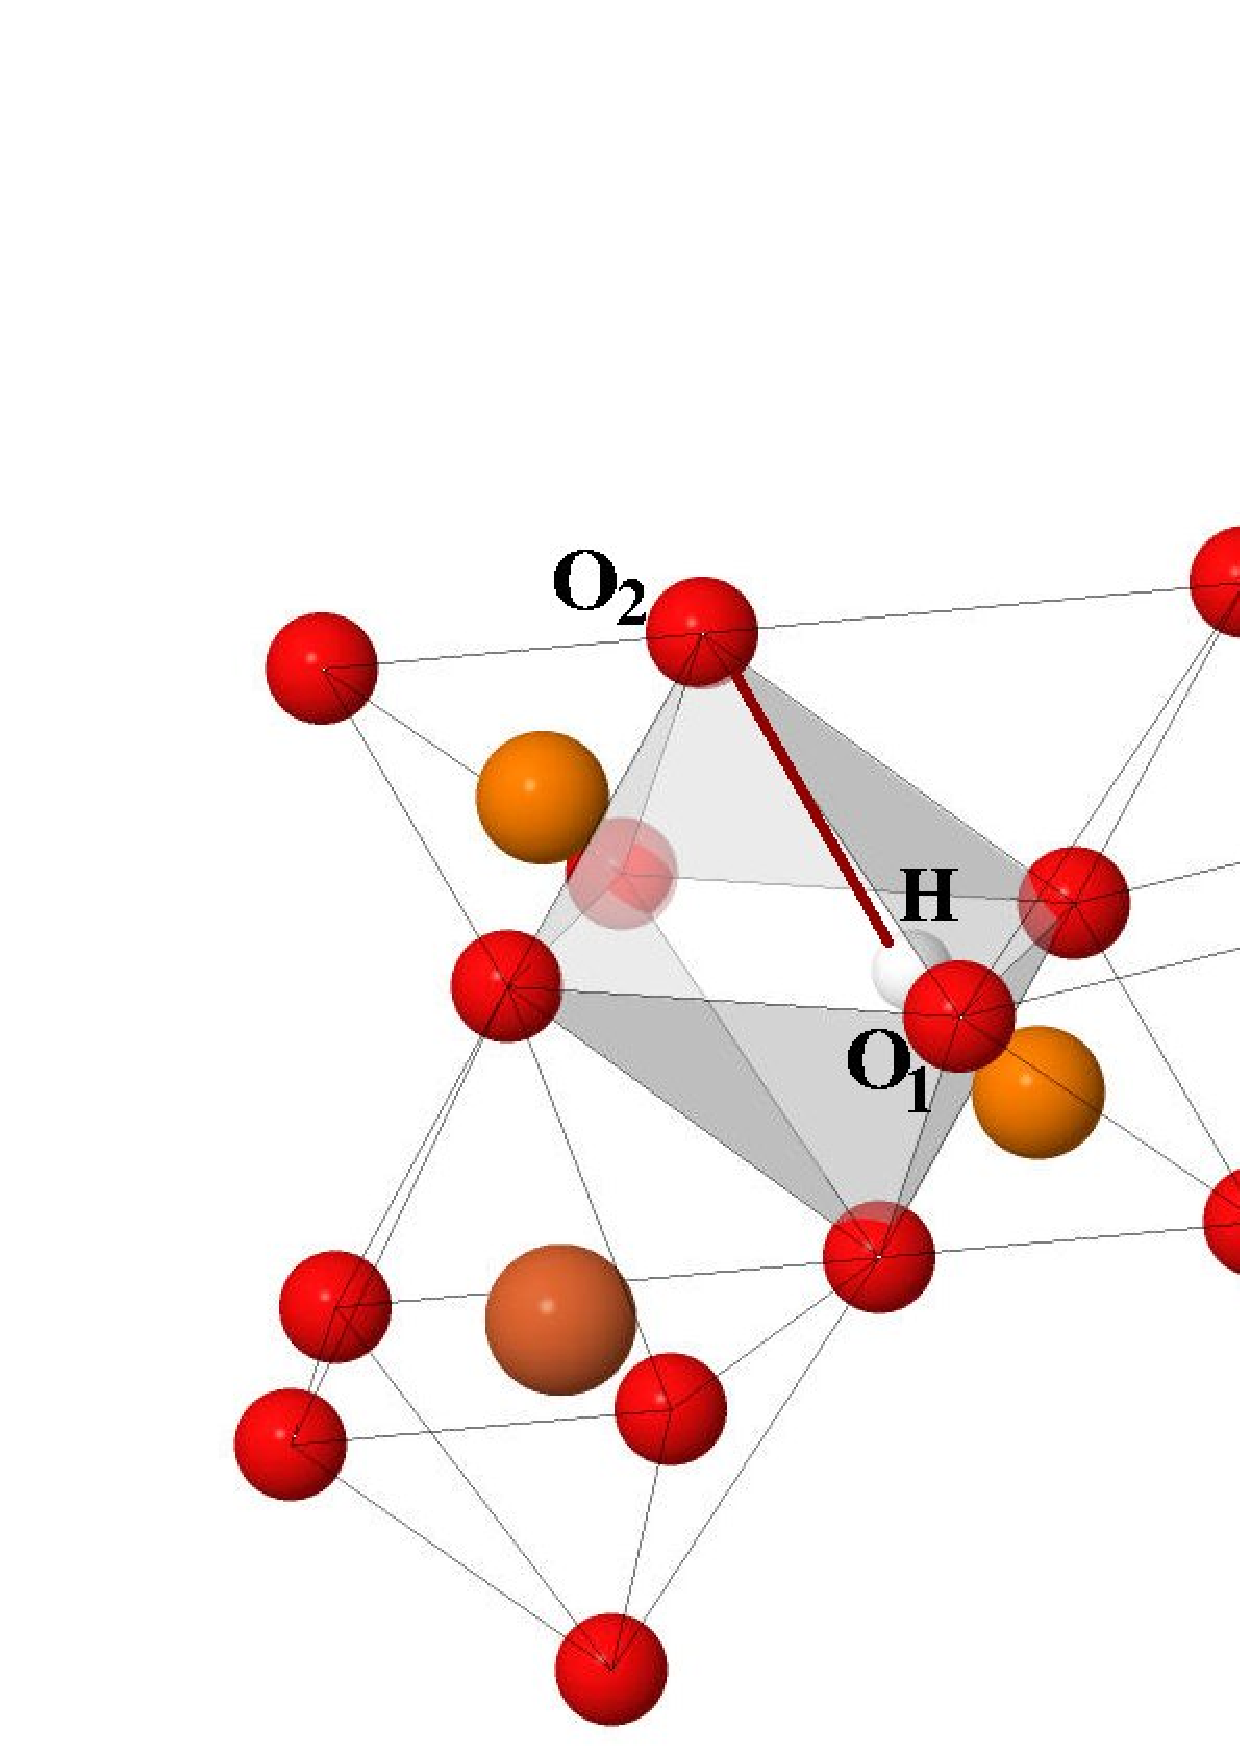
\includegraphics[width=0.9\linewidth]{pictures/oct2beforeCROP.png} \\ a)}
\end{minipage}
\hfill
\begin{minipage}[ht]{0.49\linewidth}
\center{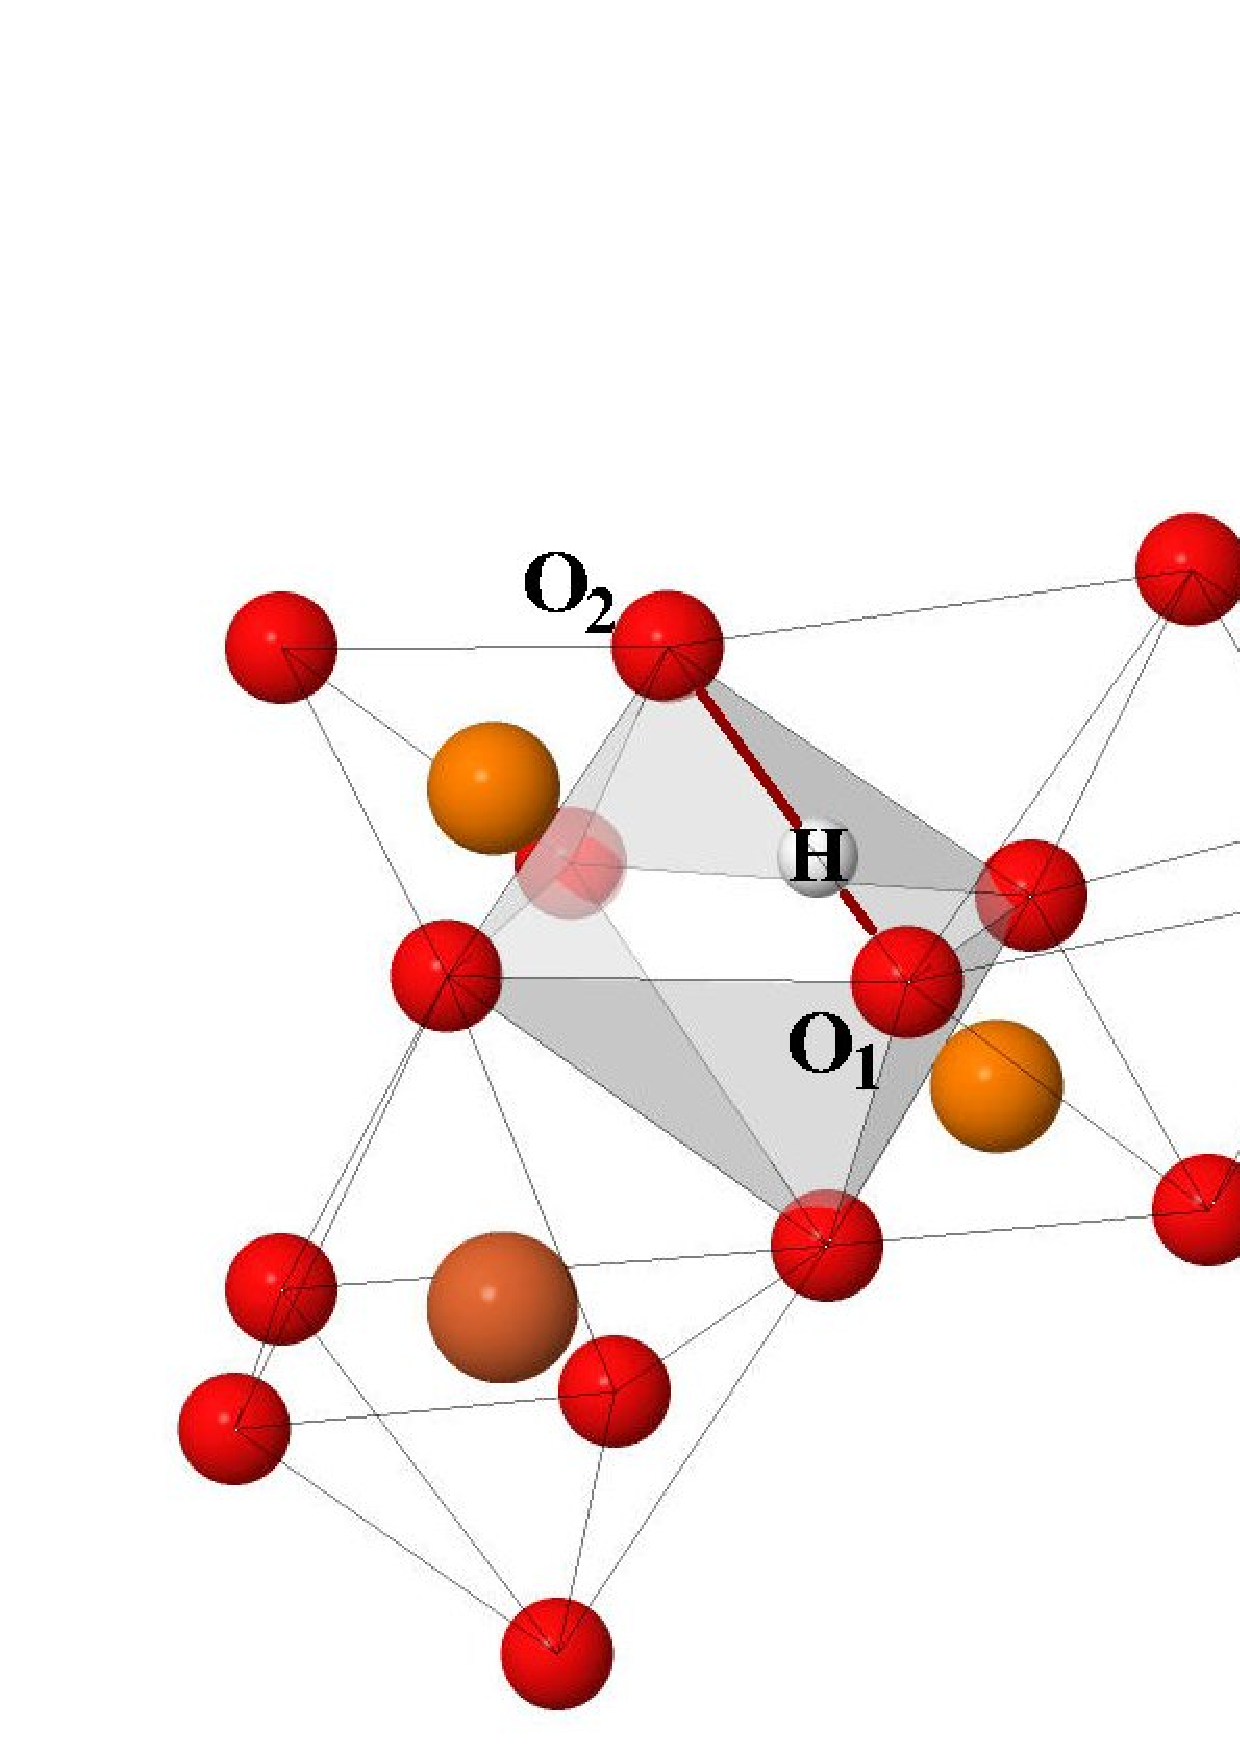
\includegraphics[width=0.9\linewidth]{pictures/oct2afterCROP.png} \\ b)}
\end{minipage}
\caption{Position of H atom in octahedral void before (a) and after (b) structural optimization (case 2)}
\label{ris:oct2}
\end{figure}

\textbf{Interstitial hydrogen in tetrahedral voids of ideal LiFePO$_4$}

Two stable hydrogen positions in tetrahedral void of LiFePO$_4$ structure were discovered.
In the first case the H atom was placed in the center of tetrahedral void (Figure~\ref{ris:tet1} a). After relaxation, the distances between the interstitial H atom and other atoms changed for H-O1 from 1.84{~\AA} to 2.54{~\AA}, for H-O2 from 1.69{~\AA} to 1.54{~\AA}, and for H-Fe from 2.09{~\AA} to 1.48{~\AA} (Figure~\ref{ris:tet1}). It is important to note the change of distance between O2 atom and neighboring iron increases from 2.21{~\AA} to 2.98{~\AA}. The formation energy of such defect is equal to 3.05~eV.

In the second case interstitial hydrogen was placed near the iron with the H-O$_1$ distance equal to 1.2{~\AA}, which have changed to 0.99{~\AA} after relaxation of the atomic positions (Figure~\ref{ris:tet2}). The formation energy of such defect is equal to 3.15 eV.	


\begin{figure}[h!]
\begin{minipage}[h]{0.49\linewidth}
\center{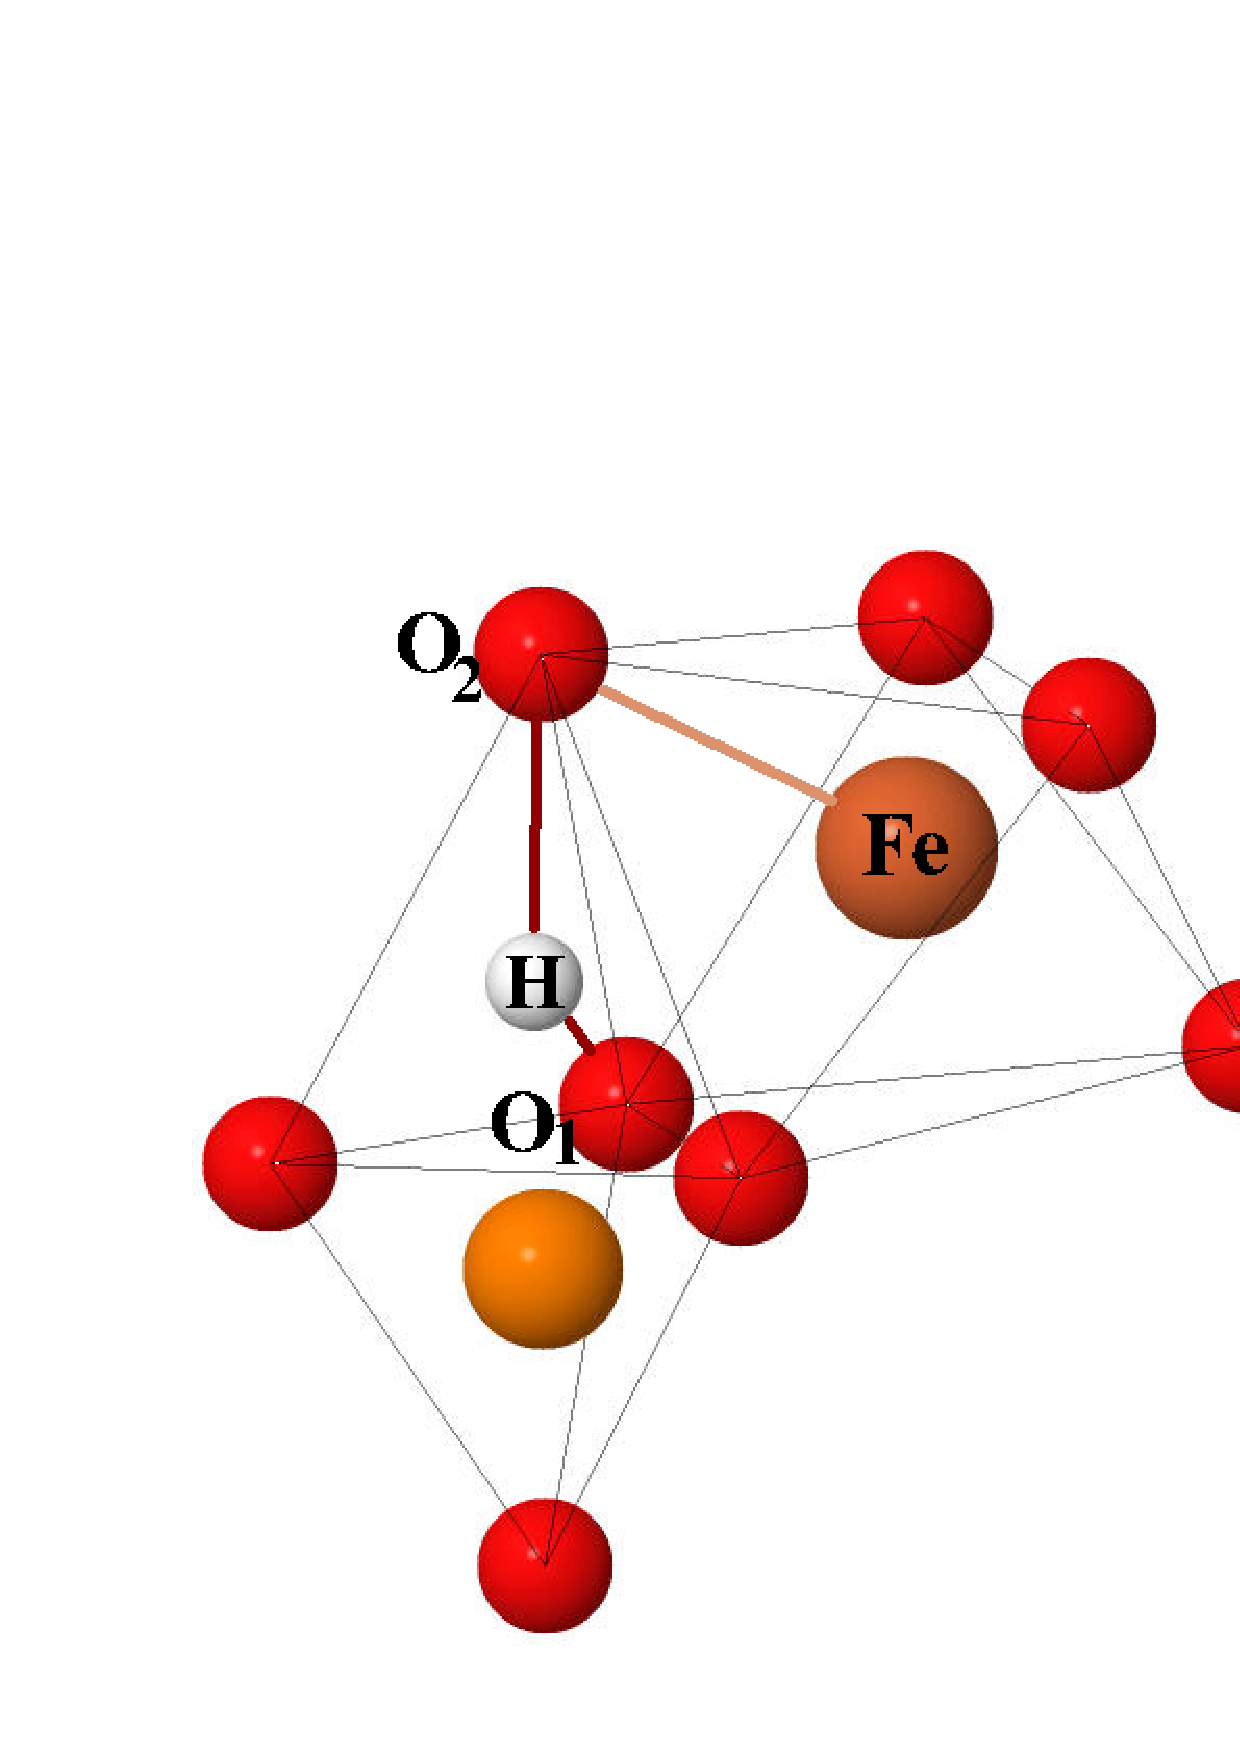
\includegraphics[width=0.9\linewidth]{pictures/tet1beforeCROP.png} \\ a)}
\end{minipage}
\hfill
\begin{minipage}[ht]{0.49\linewidth}
\center{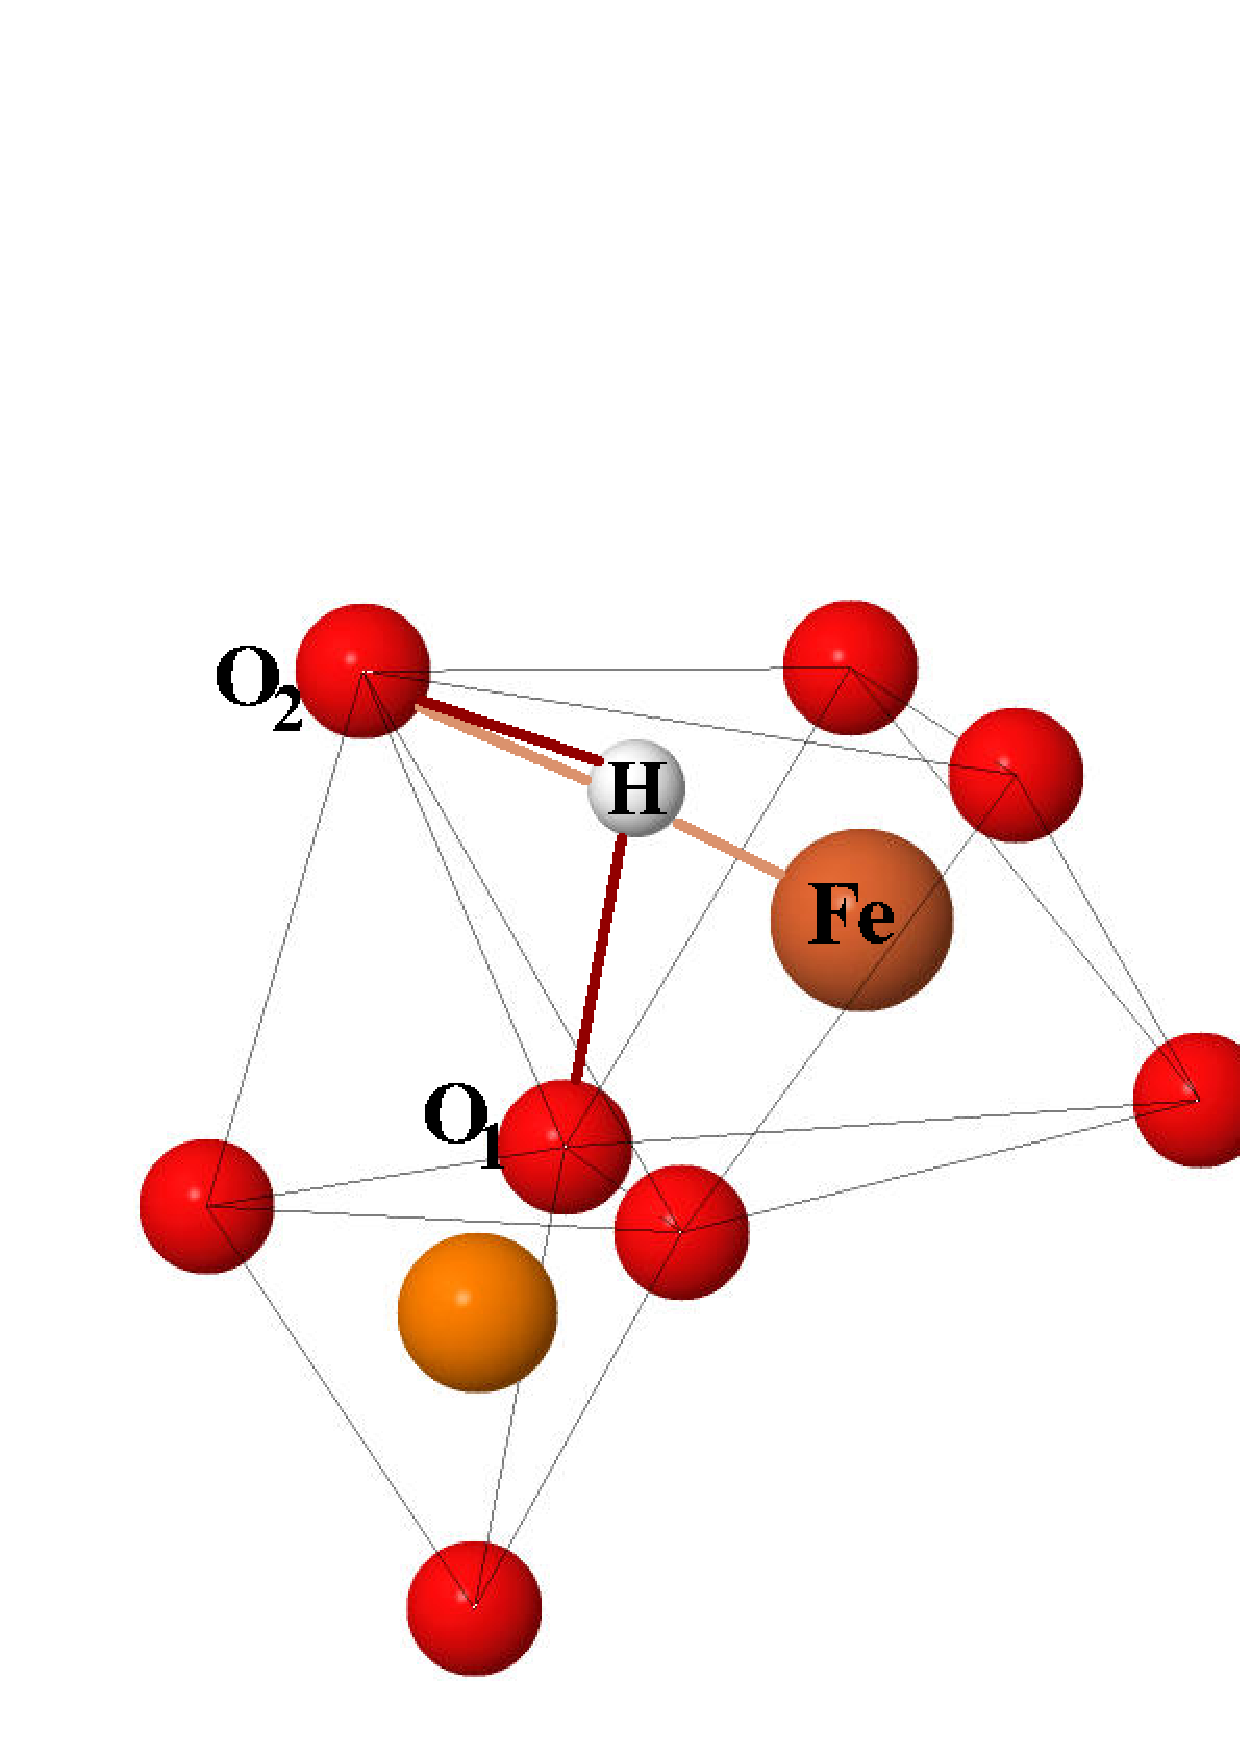
\includegraphics[width=0.9\linewidth]{pictures/tet1afterCROP.png} \\ b)}
\end{minipage}
\caption{Position of H atom in tetrahedral void before (a) and after (b) structural optimization (case 1)}
\label{ris:tet1}
\end{figure}

\begin{figure}[h!]
\begin{minipage}[h]{0.49\linewidth}
\center{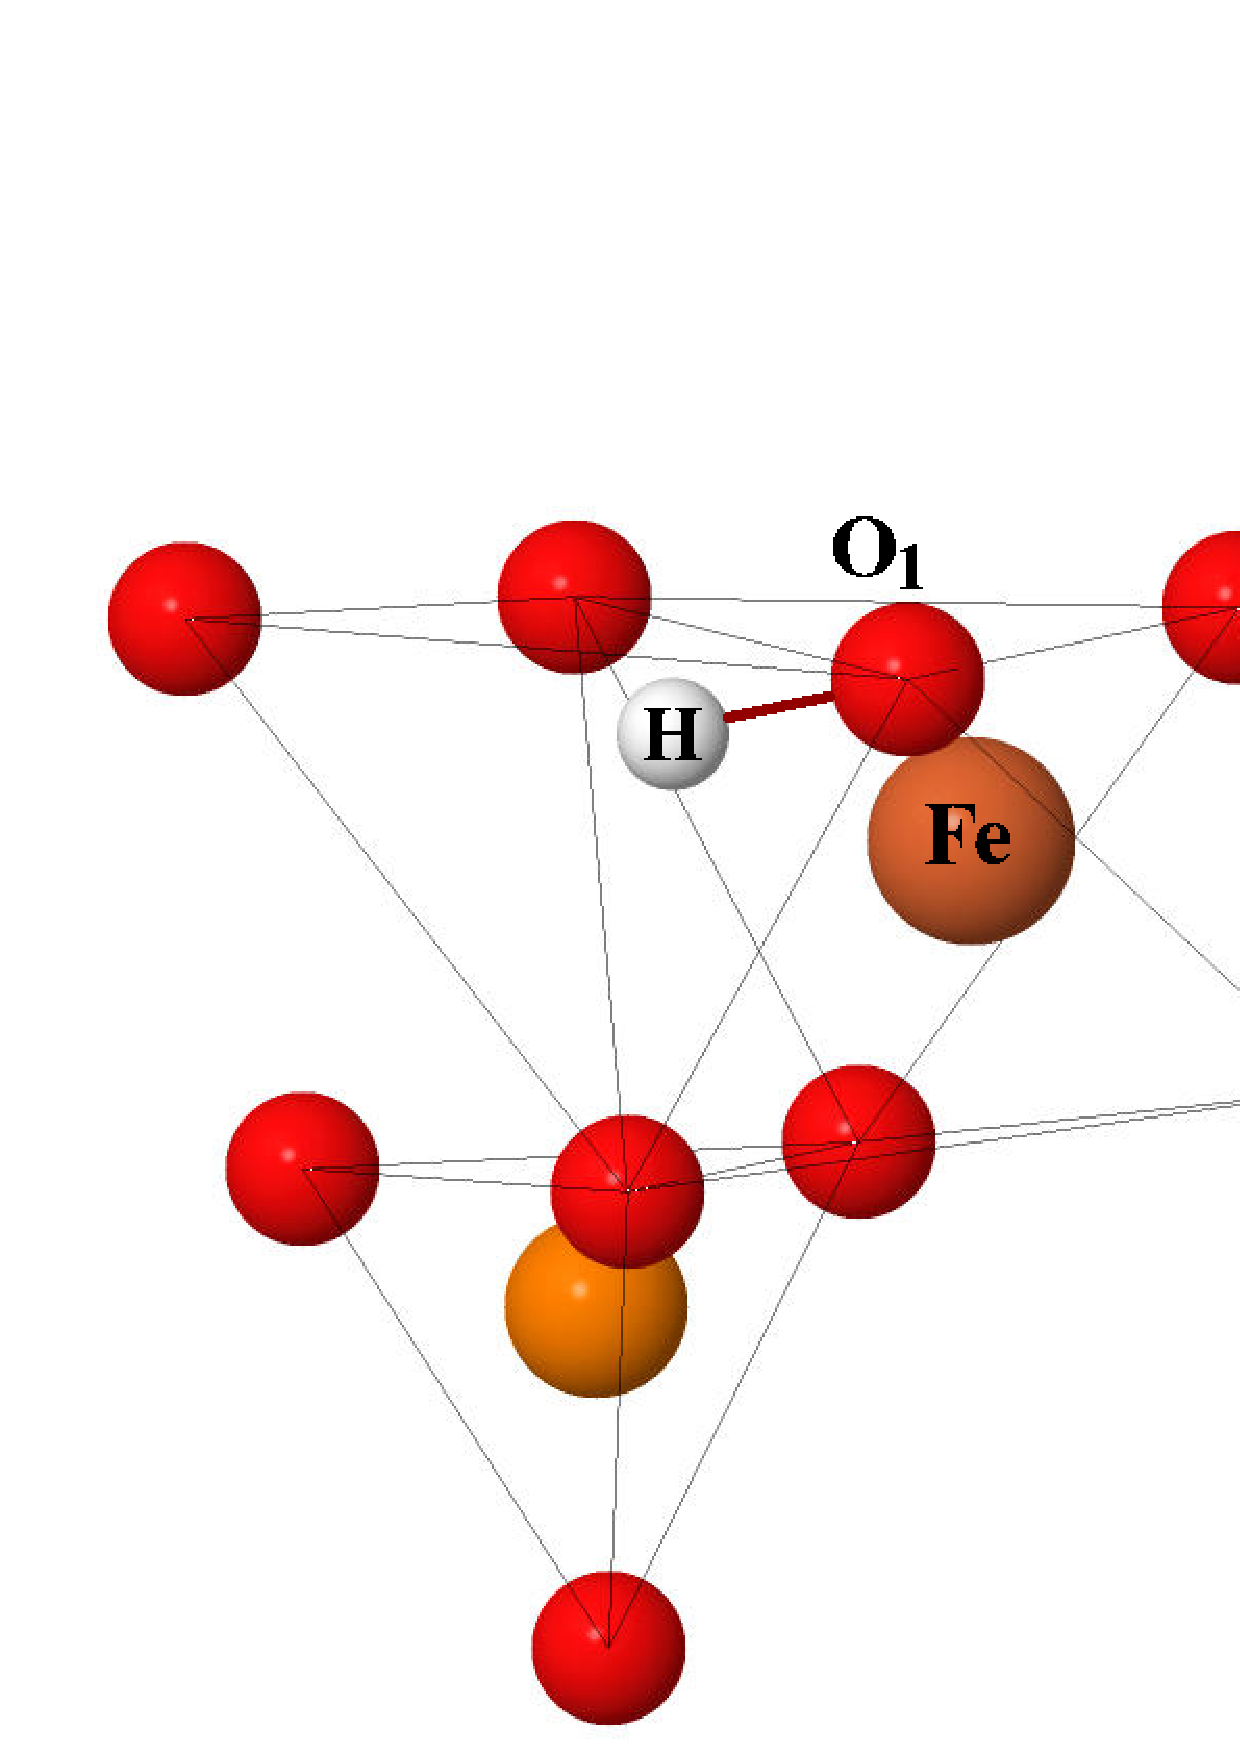
\includegraphics[width=0.9\linewidth]{pictures/tet2beforeCROP.png} \\ a)}
\end{minipage}
\hfill
\begin{minipage}[h]{0.49\linewidth}
\center{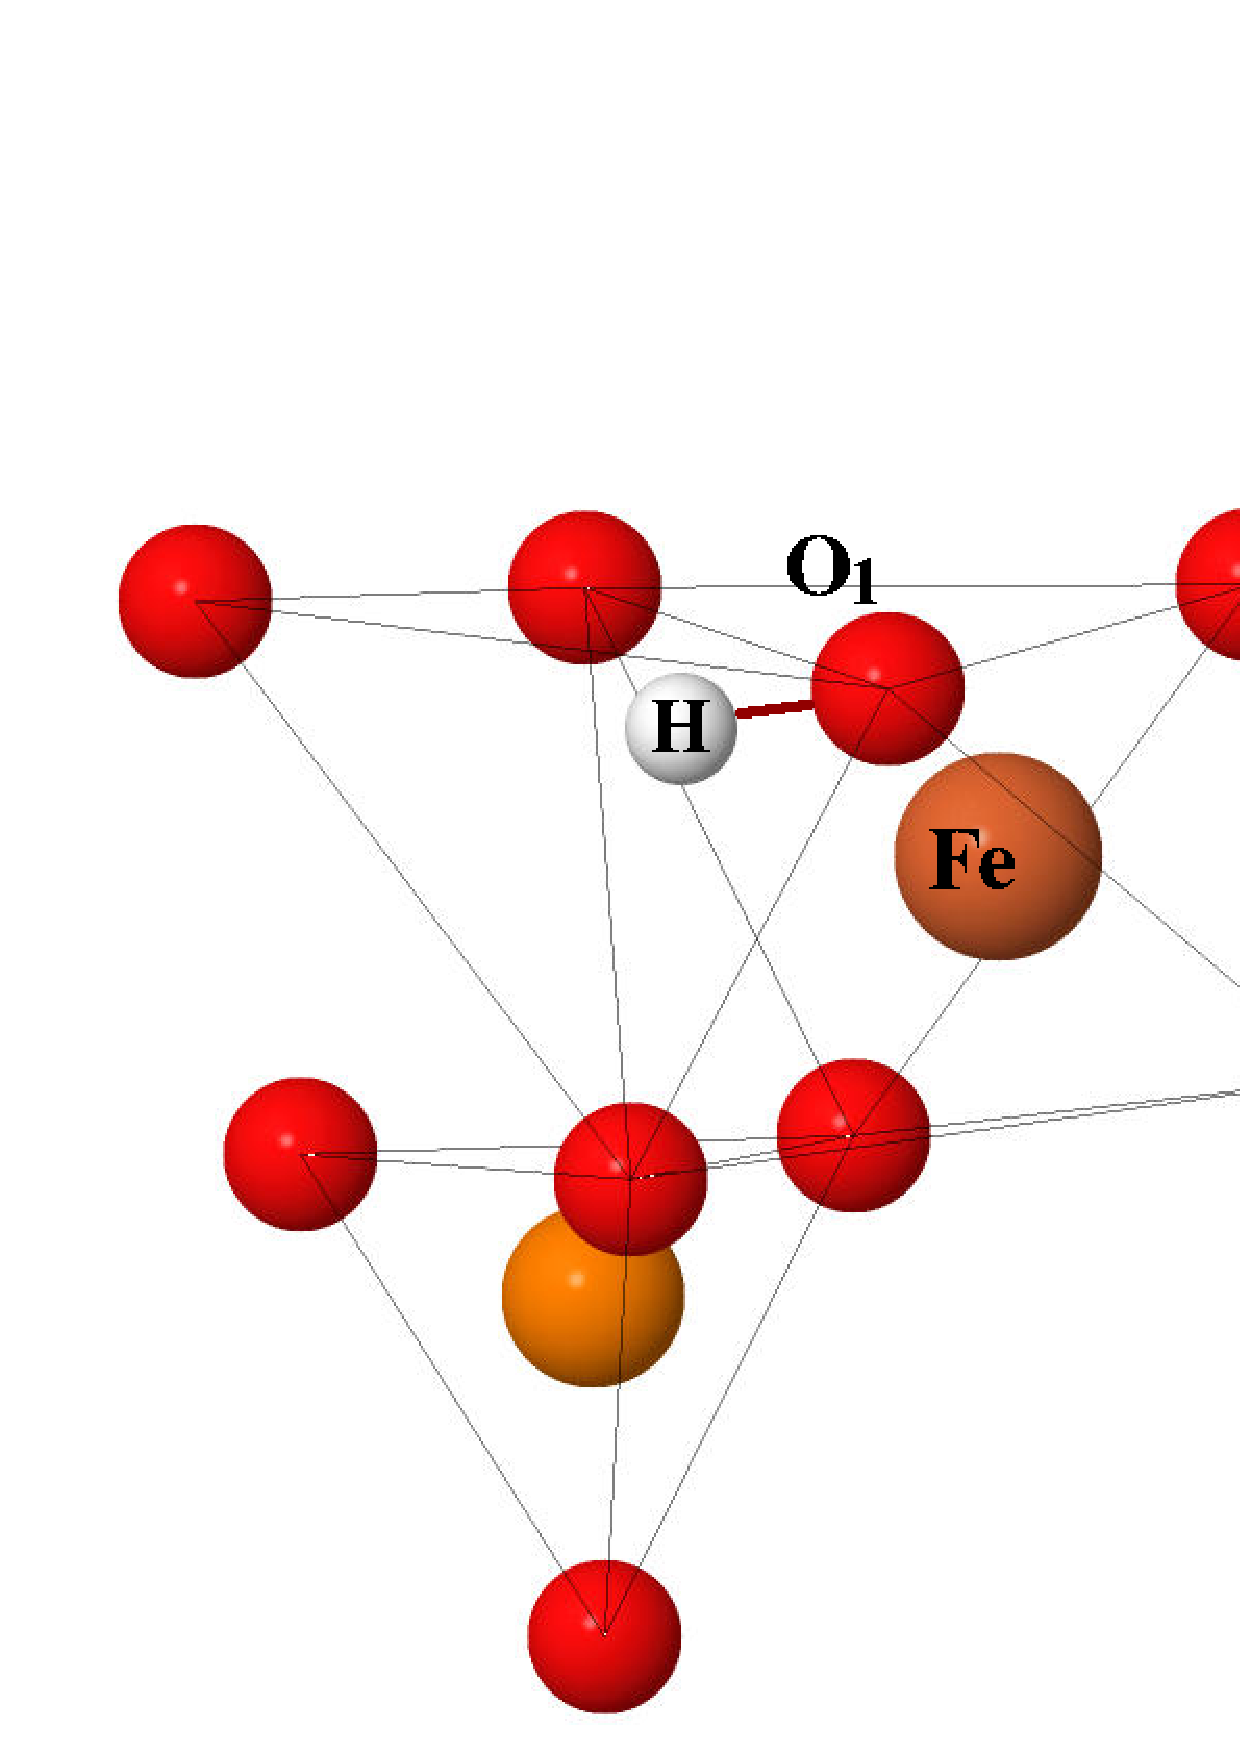
\includegraphics[width=0.9\linewidth]{pictures/tet2afterCROP.png} \\ b)}
\end{minipage}
\caption{Position of H atom in tetrahedral void before (a) and after (b) structural optimization (case 2)}
\label{ris:tet2}
\end{figure}

% The summary of the interstitial defect study is presented in Table \ref{tabular:intersti}. According to this data, the interstitial defects in any void sites are unfavorable. Thus, the substitution defects are more relevant for the further investigation. 

\par\bigskip
\textbf{Substitution of lithium by hydrogen in LiFePO$_4$}

The substitution of lithium by hydrogen  was considered. In this case the change of the hydrogen position and the relative distances are shown in Figure~\ref{ris:Li1H}. After the atomic relaxation the distance between the hydrogen atom and neighboring oxygen atom H-O$_1$ has been changing from 0.99{~\AA} to 1.00{~\AA}, Figure~\ref{ris:Li1H}. The formation energy of Li/1H substitution defect was calculated according to equation~(\ref{eq:Livac}). The corresponding formation energy of such substitution defect was equal to 0.18~eV for oxygen chemical potential $\mu(O_2)$= --11.52~eV and 0.38~eV for $\mu(O_2)$= --13.1 eV, Table~\ref{tabular:intersti}.

\begin{equation}
\label{eq:Livac}
\mu(\rm Li_{vacancy})=E(\rm Li_{1-x}Vac_{x}FePO_4)-E(\rm LiFePO_4)+\mu(\rm Li)-\mu(\rm H) 
\end{equation}

\begin{figure}[h]
\begin{minipage}[h]{0.49\linewidth}
\center{\includegraphics[width=0.9\linewidth]{pictures/Li1HbeforeCROP.png} \\ a)}
\end{minipage}
\hfill
\begin{minipage}[h]{0.49\linewidth}
\center{\includegraphics[width=0.9\linewidth]{pictures/Li1HafterCROP.png} \\ b)}
\end{minipage}
\caption{Changes of substitution of lithium by hydrogen structural optimization}
\label{ris:Li1H}
\end{figure}

\par\bigskip
\textbf{Substitution of iron by hydrogen in LiFePO$_4$}

The next considered substitution defect is hydrogen in place of iron atom. According to the oxidation state of iron in LiFePO$_4$, two H should replace one Fe to achieve initial charge balance. The distinction in the distance between neighboring atoms is presented in Figure~\ref{ris:Fe2H}. In this case the distances between first hydrogen and oxygen atoms H$_1$--O$_1$ were changed from 1.25{~\AA} to 1.00{~\AA}; H$_1$--O$_3$ -- from 2.71{~\AA} to 2.00{~\AA}. The distances between second hydrogen and neighboring oxygen atoms were changed for H$_2$--O$_2$ from 1.20{~\AA} to 0.99{~\AA}, for H$_2$--O$_3$ from 2.27{~\AA} to 1.94{~\AA}. The formation energy of this defect is calculated according to the equation~(\ref{eq:Fevac}) and is equal to 0.30 eV for oxygen chemical potential $\mu(O_2)$= --11.52 eV and 0.50 eV for $\mu(O_2)$= --13.1 eV, Table~\ref{tabular:intersti}.

\begin{equation}
\label{eq:Fevac}
E(\rm Fe_{vacancy})=\frac{1}{2}(E(\rm LiFe_{1-x}Vac_{x}PO_4)-E(\rm LiFePO_4)+\mu(\rm Fe)-2\mu(\rm H)) 
\end{equation}

\begin{figure}[h]
\begin{minipage}[h]{0.49\linewidth}
\center{\includegraphics[width=0.9\linewidth]{pictures/Fe2HbeforeCROP.png} \\ a)}
\end{minipage}
\hfill
\begin{minipage}[h]{0.49\linewidth}
\center{\includegraphics[width=0.9\linewidth]{pictures/Fe2HafterCROP.png} \\ b)}
\end{minipage}
\caption{Changes of substitution of iron by two hydrogen after structural optimization}
\label{ris:Fe2H}
\end{figure}

\begin{table}[h]
\footnotesize{
\caption{Calculated formation energies of interstitial and substitution OH defects in LiFePO$_4$}
\label{tabular:intersti}
\begin{center}
\begin{tabular}{|c|c|c|c|}
\hline
& & & \\
Interstitial & E$_{form}$, eV           &  E$_{form}$, eV & E$_{form}$, eV \\
defect      & (GGA)                     &  (GGA) & (GGA+U) \\
            & $\mu(O_2)$=-11.52 eV      &  $\mu(O_2)$=-13.1 eV & $\mu(O_2)$=-13.1 eV \\
\hline
& & & \\
Oct1 & 3.35 & 2.96 & -- \\ 
\hline
& & & \\
Oct2 & 3.22 & 2.83 & -- \\ 
\hline
& & & \\
Tet1 &  3.05 & 2.66 & -- \\ 
\hline
& & & \\
Tet2 &  3.15 & 2.76 & -- \\ 
\hline
& & & \\
Li/1H & 0.18 & 0.38 & 0.89 \\
\hline
& & & \\
Fe/2H & 0.30 & 0.50 & 0.88 \\
\hline
\end{tabular}
\end{center}
}
\end{table}

\par
According to the data from Table~\ref{tabular:intersti}, the value of each substitution defect formation energy notably depends on the calculation method: GGA without Hubbard correction gives lower formation energy in comparison with GGA+U method, where the localization of d-electrons is taken into account. 

Thus, the GGA+U approach is crucial for calculating the substitution defect formation energy. At the same time, GGA without U correction is appropriate for describing structural features of point defects. 

\section{Potential energy surface of four H atoms in P vacancy}
In the case of previously considered point defects the lowest energy configurations could have been determined by local optimization algorithms. However, it the case of P replacement by four H, numerous metastable configurations requires to perform a search for global minimum. To achieve this we employ a scan of potential energy surface (PES) of H inside and near the P vacancy. The algorithm of PES construction is described in Methods section.

%  Firstly, the analytical formula of the defect formation process is shown in the equation~\ref{firstreaction}. The process of substitution defect formation has occurred through the lithium vacancy formation in water environment and consist of four hydrogen atom in the phosphorus vacancy site:

% \begin{eqnarray}
% \label{firstreaction}
%     \frac{1}{4}O_2 + \frac{1}{2}H_2O + 16 Li^{+}Fe^{2+}P^{5+}O^{2-}_4 = Li^{+}_{15}Fe^{2+}_{16}P^{5+}_{16}O^{2-}_{64} + LiOH \nonumber \\
%     \\
%     H_2O + Li^{+}_{15}Fe^{2+}_{16}P^{5+}_{16}O^{2-}_{64} + 4LiOH = H^{+}_{4}Li^{+}_{16}Fe^{2+}_{15}Fe^{3+}_{1}P^{5+}_{15}O^{2-}_{64} + Li_3PO_4 + H_2O \nonumber 
% \end{eqnarray}

The P tetrahedra in LiFePO$_4$ structure is highlighted in Figure~\ref{ris:Ploc_pic}. 
% The P atom is shown with yellow, the lithium atoms are in a purple color, the iron atoms are in a brown color, and the oxygen atoms have a red color. 
This figure shows the pseudo layered structure of LiFePO$_4$ normal to the c-axes and two planes Plane$_1$ and Plane$_2$ used further for visualization. 
As it was explained in Methods section the considered PES has spherical shape around oxygen atoms. To simplify its visualization we will show only those atoms and points that correspond to the slice with $\sim$ 2~{\AA} thickness above Plane$_1$ (Plane 1a), below Plane$_1$ (Plane 1b) and below Plane$_1$ (Plane 2)
The corresponding slices are shown in Figure~\ref{ris:planes}. 

\begin{figure}[h!]
\center{\includegraphics[width=0.9\linewidth]{pictures/plane0_atomsName.png}}
\caption{LiFePO$_4$ with highlighted P tetrahedron. The adjacent polyhedral voids can be seen.}
\label{ris:Ploc_pic}
\end{figure}

\begin{figure}[h!]
\begin{minipage}[h]{0.5\linewidth}
\center{\includegraphics[width=1.0\linewidth]{pictures/LFP_plane1_1.jpg} \\ a)}
\end{minipage}
\hfill
\begin{minipage}[ht]{0.49\linewidth}
\center{\includegraphics[width=0.9\linewidth]{pictures/LFP_plane1_2.jpg} \\ b)}
\end{minipage}
\vfill
\begin{minipage}[h]{0.49\linewidth}
\center{\includegraphics[width=0.9\linewidth]{pictures/LFP_plane2.png} \\ c)}
\end{minipage}
\caption{a) The considered slices of LFP structure used for visualization of PES.}
\label{ris:planes}
\end{figure}

As a first step the P vacancy was created by removing the P atom followed by atomic optimization. 
% Phosphorus atom can be replaced by four hydrogen atoms as it was shown above in the equations~\ref{firstreaction}. 
% In order to consider the localization of each OH-bonds the sequential review of PO$_4$/(OH)$_1$, PO$_4$/(OH)$_2$, PO$_4$/(OH)$_3$ and PO$_4$/(OH)$_4$ were discussed. 
Then the PES for H was considered around each of the four O using spherically symmetrical grid of points generated by especially developed python code, provided in Appendix A, section A.1--A.5. The total energy of H at each point was obtained from single point calculations without atomic relaxation. As will be shown further such approach is reasonable to identify the lowest energy configurations. 

Around each of the four oxygen atoms several filled and empty voids are located. In addition to Li and Fe octahedrons each oxygen is surrounded by eight tetrahedral voids (in pictures below they will be marked using gray colored numbers) and six octahedral voids (marked using black colored numbers). The P vacancy tetrahedron is highlighted using green color.

\subsection{PES for PO$_4$/O$_4$H$_1$ defect }

Our first step of PO$_4$/(OH)$_4$ defect investigation is the study of the substitution phosphorus by one hydrogen atom PO$_4$/O$_4$H$_1$. We considered 153 positions of H atom around oxygen O$_1$ (reduced coordinates: --0.046, 0.125, 0.147) changing O-H distance between 0.9{~\AA} and 1.3{~\AA}. For each structure the single point static calculation of energy was performed. The energy of each hydrogen atom in its position was calculated according to~(\ref{eq:form}) equation. The obtained slices of PES, where different energies are shown with color are provided in Figure~\ref{ris:PES1}. The dark blue colors show   the lowest energy positions of H atom and dark red colors show high energy positions. It is unfavourable for H to be near iron or lithium atoms, while it prefers to be in the tetrahedral void left after P removal (3tet) and in the octahedral void (4oct).

\begin{figure}[h!]
\begin{minipage}[h]{0.5\linewidth}
\center{\includegraphics[width=1.0\linewidth]{pictures/1H_plane1.png} \\ a)}
\end{minipage}
\hfill
\begin{minipage}[ht]{0.49\linewidth}
\center{\includegraphics[width=0.9\linewidth]{pictures/1H_plane2.png} \\ b)}
\end{minipage}
\caption{Two slices of H potential energy surface for PO$_4$/(OH)$_1$ defect. The low and high energies of H are shown with rainbow colors from dark blue to dark red.}
\label{ris:PES1}
\end{figure}

We took several lowest energy H positions in the different voids and performed atomic relaxation. 
% (except num.1, 5, and 6 black near the iron and lithium atoms due to their high equilibrium energy).
After relaxation the H atom has moved either to 3tet or 4oct voids with the latter being higher in energy by 0.4~eV. The relative energies of final configurations obtained from different initial conditions are collected  in Table~\ref{energy1}.


\begin{table}[h!]
%\normalsize{
\caption{Relative energy of hydrogen after atomic optimization of several lowest energy points of PES  for PO$_4$/(OH)$_4$ defect. The second and fourth columns show initial and final voids for H. }
\label{energy1}
\begin{center}
\begin{tabular}{|c|c|c|c|c|c|}
\hline
& & & & & \\
 \textbf{No} & \textbf{Initial $\rightarrow$ final} & \textbf{$\Delta$ E, eV} & \textbf{No} & \textbf{Initial $\rightarrow$ final} & \textbf{$\Delta$ E, eV}\\ 
\hline
& & & & & \\
\textbf{a} & \textbf{4tet $\rightarrow$ 3tet} & \textbf{0.000} & g & 5tet $\rightarrow$ 4oct & 0.416 \\
\hline
& & & & & \\
b & 7tet $\rightarrow$ 3tet & 0.001 & h & 8tet $\rightarrow$ 4oct & 0.419 \\
\hline
& & & & & \\
c & 3tet $\rightarrow$ 3tet & 0.002 & k & 4oct $\rightarrow$ 4oct & 0.420 \\
\hline
& & & & & \\
d & 3oct $\rightarrow$ 3tet & 0.002 & l & 2tet $\rightarrow$ 4oct & 0.432 \\
\hline
& & & & & \\
e & 2oct $\rightarrow$ 3tet & 0.003 & m & 1tet $\rightarrow$ 4oct & 0.483 \\
\hline
& & & & & \\
f & 6tet $\rightarrow$ 4oct & 0.415 & & & \\
\hline
\end{tabular}
\end{center}
%}
\end{table}

% The advantageous position of hydrogen atom was detected in the 4 tetrahedral site. After atomic positions relaxation the hydrogen atom moved from tetrahedral site (num.4 grey) to the edge of tetrahedral site (num.3 grey). 

In fact, the lowest energy position of H is located on the edge between tetrahedral voids 4 and 3, which is shown in  Figure~\ref{4to3}. Here, it should be noted that PES constructed with single point calculations gives quite reasonable estimation of the most favourable hydrogen position.

\begin{figure}[h]
\begin{minipage}[h]{0.3\linewidth}
\center{\includegraphics[width=1\linewidth]{pictures/4i1.jpg}}
\end{minipage}
\hfill
\begin{minipage}[h]{0.3\linewidth}
\center{\includegraphics[width=1\linewidth]{pictures/4o1.jpg}} 
\end{minipage}
\hfill
\begin{minipage}[h]{0.3\linewidth}
\center{\includegraphics[width=1\linewidth]{pictures/4o2.jpg}} 
\end{minipage}
\caption{Relaxation of H from tetrahedral void 4 to tetrahedral void 3. Left figure: before relaxation; Center and right figures: after relaxation.}
\label{4to3}
\end{figure}

In the same manner the relaxation of H is observed for octahedral voids (number 2 and 3 black) and tetrahedral voids (number 3 and 7 grey). The H movement from tetrahedral site (number 7 grey) to the tetrahedron with P vacancy (number 3 grey) is shows in Figures~\ref{7to31} and ~\ref{7to3} using different slices.  These hydrogen atom position have higher energy than in the case of 3tet. Hydrogen atoms from other positions: the octahedral void (num.4 black) and tetrahedral sites with (num.1, 2, 5, 6, and 8 grey) have even higher energy. In these cases atoms from their initial positions move to the boundary with octahedral void (num.4 black), Table~\ref{energy1}.

\begin{figure}[h!]
\begin{minipage}[h]{0.5\linewidth}
\center{\includegraphics[width=0.9\linewidth]{pictures/7i1.jpg}}
\end{minipage}
\hfill
\begin{minipage}[h]{0.5\linewidth}
\center{\includegraphics[width=0.9\linewidth]{pictures/7o1.jpg}} 
\end{minipage}
\caption{Movement of hydrogen atom from 7 tetrahedral void to 3 tetrahedral void. Pictures on the left side -- before relaxation; pictures in the right side -- after relaxation.}
\label{7to31}
\end{figure}

\begin{figure}[h!]
\begin{minipage}[h]{0.5\linewidth}
\center{\includegraphics[width=0.9\linewidth]{pictures/7i2.jpg}} 
\end{minipage}
\hfill
\begin{minipage}[h]{0.5\linewidth}
\center{\includegraphics[width=0.9\linewidth]{pictures/7o2.jpg}} 
\end{minipage}
\caption{Movement of hydrogen atom from 7 tetrahedral void to 3 tetrahedral void -- one of more stable position: pictures on the left side -- before relaxation; pictures in the right side -- after relaxation in the plane 3}
\label{7to3}
\end{figure}

According to calculated results, some outcomes can be concluded:

1. Potential energy surface scan of hydrogen grid distribution shows the appropriate and inappropriate positions of hydrogen in the phosphorus deficient LiFePO$_4$ material. 
2. PES scan is a useful tool for  prediction of possible equilibrium hydrogen positions;
2. According to further calculation of atomic positions relaxation the equilibrium sites of hydrogen atom in phosphorus vacancy tetrahedron were confirmed;
3. The movement of hydrogen atom between tetrahedral sites (num.4 and 3 grey) was established as a more appropriate due to its low formation energy. 

%\newpage
\subsection{PES for PO$_4$/O$_4$H$_2$ defect}

As a next step we constructed a PES for hydrogen  around second oxygen of the phosphorus-defective tetrahedron, while the first hydrogen was fixed in its equilibrium position (from the first study of PO$_4$/(OH)$_1$). The obtained PES slices are shown in Figure~\ref{HinO1and2}. 

\begin{figure}[h!]
\begin{minipage}[h]{0.5\linewidth}
\center{\includegraphics[width=1\linewidth]{pictures/2OPlane1CUT4.jpg}}
\end{minipage}
\hfill
\begin{minipage}[h]{0.5\linewidth}
\center{\includegraphics[width=1\linewidth]{pictures/2OPlane2CUT4.jpg}} 
\end{minipage}
\caption{Hydrogen distribution around second oxygen in phosphorus-defective tetraherdal site (8 grey number)}
\label{HinO1and2}
\end{figure}

The hydrogen atoms inside the phosphorus vacancy tetrahedral site (num.8 grey in Pane 2) have lower energy in comparison to other outside hydrogen atoms (for example, near iron atom in the Plane 1 figure). The atomic positions relaxation was provided for each LiFePO$_4$ system with two hydrogen atoms: near first oxygen in its equilibrium position and second oxygen in various position. The formation energy of each site of the second hydrogen was calculated and the Table~\ref{energy2} was completed.

\begin{table}[h!]
%\scriptsize{
\caption{Energy of hydrogen in different polyhedral sites around second oxygen}
\label{energy2}
\begin{center}
\begin{tabular}{|c|c|c|c|c|c|}
\hline
& & & & &\\
 \textbf{No} & \textbf{Initial $\rightarrow$ final} & \textbf{$\Delta$ E, eV} & \textbf{No} & \textbf{Initial $\rightarrow$ final} & \textbf{$\Delta$ E, eV}\\ 
\hline
& & & & &\\
\textbf{a} & \textbf{5oct $\rightarrow$ 7tet} & \textbf{0.0000} & h & 3tet $\rightarrow$ 6tet & 0.0011 \\
\hline
& & & & &\\
b & 4oct $\rightarrow$ 6tet & 0.0003 & k & 2tet $\rightarrow$ 7tet & 0.0012 \\
\hline
& & & & &\\
c & 1oct $\rightarrow$ 7tet & 0.0003 & l & 6oct $\rightarrow$ 6tet/8tet & 0.0022\\
\hline
& & & & &\\
d & 8tet $\rightarrow$ 6tet/8tet & 0.0007 & m & 4tet $\rightarrow$ 1tet & 0.7166\\
\hline
& & & & &\\
e & 2oct $\rightarrow$ 6tet & 0.0007 & n & 5tet $\rightarrow$ 1tet & 0.7185\\
\hline
& & & & &\\
f & 7tet $\rightarrow$ 7tet & 0.0008 & o & 1tet $\rightarrow$ 1tet & 0.7185 \\
\hline
& & & & &\\
g & 6tet $\rightarrow$ 6tet/8tet & 0.0011 & & & \\
\hline
\end{tabular}
\end{center}
%}
\end{table}

The movement of two hydrogen atoms from initial positions to final advantageous positions after the atomic relaxation calculation is presented in the Figure~\ref{O2Finitialfinal}.

According to this information, some outcomes can be concluded:

1. The hydrogen atom moves from the octahedral void (num.5 black) to the tetrahedral void (num.7 grey) and has the lowest formation energy in comparison to other hydrogen positions;

2. The similar low-energy state can be observed for hydrogen atoms in the octahedral voids (num.1, 2, 4 black)  and in the tetrahedral voids num.2, 3, 6, 7, 8 grey), which have moved to the edge of the tetrahedral voids (num.6, 7 and 8 grey) during the relaxation of atomic structure;

3. The energetically-advantageous position can be also observed in the tetrahedral void (num.4 grey), where the hydrogen atoms from the tetrahedral voids (num.1, 4, and 5 grey) have been moved to more stable positions.

\begin{figure}[h!]
\begin{minipage}[h]{0.5\linewidth}
\center{\includegraphics[width=1\linewidth]{pictures/2O5blackinitial.jpg}}
\end{minipage}
\hfill
\begin{minipage}[h]{0.5\linewidth}
\center{\includegraphics[width=1\linewidth]{pictures/2O5blackfinal.jpg}} 
\end{minipage}
\caption{The most stable positions of two H atoms in the P vacancy before and after relaxation (grey number 8).}
\label{O2Finitialfinal}
\end{figure}

\subsection{PES for PO$_4$/O$_4$H$_3$ defect }
 
The study of hydrogen atoms distribution around the third oxygen atom in phosphorus-defective LiFePO$_{4}$ structure with the presence of two hydrogen near the first and second oxygen (from 1 and 2 steps of investigation) is described in the current paragraph.

The constructed PES is presented in Figure~\ref{HinO1,2and3}. According to PES, the assumption about an advantageous position of the third hydrogen atom near tetrahedral site (num.2 grey) and the octahedral site (num.5 black) can be made.

The stable positions and resulting relative energies are collected in Table~\ref{energy3}.

\begin{figure}[h]
\begin{minipage}[h]{0.5\linewidth}
\center{\includegraphics[width=0.9\linewidth]{pictures/3OPlane1.jpg}}
\end{minipage}
\hfill
\begin{minipage}[h]{0.5\linewidth}
\center{\includegraphics[width=1.02\linewidth]{pictures/3OPlane2.jpg}} 
\end{minipage}
\caption{Hydrogen PES around third oxygen in the phosphorus-defective tetraherdal void (number 2 grey)}
\label{HinO1,2and3}
\end{figure}

% The positions of third hydrogen atoms depending on their initial distribution were found after the relaxation of atomic positions. This information is formed a Table~\ref{energy3}, 

Several conclusions can be formulated from Table~\ref{energy3}:

1. Structure with lower energy is formed with the third atom, which is moved from the octahedral void (num.2 black) to the edge between the tetrahedral void (num.2 grey) and the octahedral void (num.3 black). 

2. Another advantageous position of the third hydrogen atom can be observed, when hydrogen moved between two octahedral void (from num.6 black to num.5 black).

3. Generally, the more appropriate places of third hydrogen atom locations are the tetrahedral void (num.2 grey) and the octahedral void (num.5 black), which is confirmed by Table~\ref{energy3} after relaxation and non-relaxation information. 

\begin{table}[h]
%\scriptsize{
\caption{Energy of hydrogen in different polyhedral sites around third oxygen}
\label{energy3}
\begin{center}
\begin{tabular}{|c|c|c|c|c|c|}
\hline
& & & & & \\
 \textbf{No} & \textbf{Initial $\rightarrow$ final} & \textbf{$\Delta$ E, eV} & \textbf{No} & \textbf{Initial $\rightarrow$ final} & \textbf{$\Delta$ E, eV}\\ 
\hline
& & & & & \\
\textbf{a} & \textbf{2oct $\rightarrow$ 2tet/3oct} & \textbf{0.000} & h & 3oct $\rightarrow$ 2tet/3oct & 0.514 \\
\hline
& & & & & \\
b & 6oct $\rightarrow$ 5oct & 0.190 & k & 3tet $\rightarrow$ 3oct & 0.514 \\
\hline
& & & & & \\
c & 1oct $\rightarrow$ 2tet/4tet & 0.511 & l & 4oct $\rightarrow$ 2tet/3oct & 0.515 \\
\hline
& & & & & \\
d & 6tet $\rightarrow$ 2tet/3oct & 0.512 & m & 8tet $\rightarrow$ 5oct & 0.734 \\
\hline
& & & & & \\
e & 2tet $\rightarrow$ 2tet/3oct & 0.512 & n & 5oct $\rightarrow$ 5oct & 0.738 \\
\hline
& & & & & \\
f & 4tet $\rightarrow$ 2tet & 0.512 & o & 7tet $\rightarrow$ 5oct & 0.740\\
\hline
& & & & & \\
g & 1tet $\rightarrow$ 1oct & 0.514 & p & 5tet $\rightarrow$ 5oct & 0.902 \\
\hline
\end{tabular}
\end{center}
%}
\end{table}

In Figure~\ref{O3Finitialfinal}, the movement of third atom between initial and final positions is presented.

\begin{figure}[h!]
\begin{minipage}[h]{0.5\linewidth}
\center{\includegraphics[width=1\linewidth]{pictures/3Obefore2black.jpg}}
\end{minipage}
\hfill
\begin{minipage}[h]{0.5\linewidth}
\center{\includegraphics[width=1\linewidth]{pictures/3Oafter2black.jpg}} 
\end{minipage}
\caption{Hydrogen movement to stable position around third oxygen in phosphorus-defective LiFePO$_4$}
\label{O3Finitialfinal}
\end{figure} 

%\newpage
\subsection{PES for PO$_4$/(OH)$_4$ }

The last stage of the substitution of phosphorus by four hydrogen defect investigation is presented in the Figure~\ref{HinO1,2,3and4}. 

\begin{figure}[h]
\begin{minipage}[h]{0.5\linewidth}
\center{\includegraphics[width=0.93\linewidth]{pictures/4OPlane1.jpg}}
\end{minipage}
\hfill
\begin{minipage}[h]{0.5\linewidth}
\center{\includegraphics[width=1\linewidth]{pictures/4OPlane2.jpg}} 
\end{minipage}
\caption{Hydrogen distribution around fourth oxygen in phosphorus-defective tetrahedral site (2 grey number)}
\label{HinO1,2,3and4}
\end{figure}

According to the information about the formation energy of each hydrogen atom from Table~\ref{energy4}, the conclusion about the place of appropriate hydrogen atom localization can be formulated. There are two octahedral sites (with 3 and 5 grey numbers), close to which the movement of the fourth hydrogen is advantageous.  

\begin{table}[h]
%\scriptsize{
\caption{Energy of hydrogen in different polyhedra positions around fourth oxygen}
\label{energy4}
\begin{center}
\begin{tabular}{|c|c|c|c|c|c|}
\hline
& & & & &\\
\textbf{No} & \textbf{Initial $\rightarrow$ final} & \textbf{$\Delta$ E, eV} & \textbf{No} & \textbf{Initial $\rightarrow$ final} & \textbf{$\Delta$ E, eV}\\ 
\hline
& & & & &\\
\textbf{a} & \textbf{3oct $\rightarrow$ 3oct} & \textbf{0.000} & g & 1tet $\rightarrow$ 4oct/5tet & 0.184 \\
\hline
& & & & &\\
b & 5oct $\rightarrow$ 5oct & 0.001 & h & 7tet $\rightarrow$ 3oct & 0.307 \\
\hline
& & & & &\\
c & 5tet $\rightarrow$ 2tet/1oct & 0.056 & k & 3tet $\rightarrow$ 3oct & 0.309 \\
\hline
& & & & &\\
d & 4oct $\rightarrow$ 1oct & 0.130 & l & 2tet $\rightarrow$ 2tet/1oct & 0.921 \\
\hline
& & & & &\\
e & 8tet $\rightarrow$ 2tet/1oct & 0.181 & m & 6tet/1oct & 1.212 \\
\hline
& & & & &\\
f & 4tet $\rightarrow$ 4tet/2tet & 0.181 & & &\\
\hline
\end{tabular}
\end{center}
%}
\end{table}

\begin{figure}[h!]
\begin{minipage}[h]{0.5\linewidth}
\center{\includegraphics[width=1\linewidth]{pictures/4Obefore.jpg}}
\end{minipage}
\hfill
\begin{minipage}[h]{0.5\linewidth}
\center{\includegraphics[width=1\linewidth]{pictures/4Oafter.jpg}} 
\end{minipage}
\caption{Hydrogen movement to stable position around fourth oxygen in phosphorus-defective LFP}
\label{O4Finitialfinal}
\end{figure}

\newpage
Thus, the movement of the fourth hydrogen atom is presented in Figure~\ref{O4Finitialfinal} with corresponding between initial and final configuration of LiFePO$_{4}$ structure with phosphorus defect. The result of the calculation with atomic position relaxation shows the significant movement of the first hydrogen atom in comparison to its initial state. At the same time the fourth atom takes its place approximately along the O--O bond within phosphorus vacancy tetrahedron. As a result, the second, third, and fourth hydrogen atom under estimation took their place within the tetrahedron area of phosphorus vacancy site, while the first hydrogen atom localized in the neighboring octahedral void.

\par\bigskip
\section{Formation energy of OH defects in LiFePO$_4$}
%\textbf{Substitution of phosphorus by hydrogen in LiFePO$_4$}

As soon as the substitution of phosphorus by four hydrogen atoms defect structure was considered, its formation energy was compared with other defects, which were presented in previous sections. Additionally, if one phosphorus atom P$^{5+}$ is removed from its stable position, five iron atoms in the neighboring area changes their oxidation state from Fe$^{2+}$ to Fe$^{3+}$. Then there can be two scenarios of substitution defects of phosphorus: four or five hydrogen atoms can be placed in the vacancy site, equation~(\ref{eq:Pvacancy}). 
Four atoms of hydrogen can build OH bonds with each of the oxygen in the tetrahedral environment. In this case just one iron atom will change its oxidation state. To achieve charge balance and taking into account the valency of a phosphorus atom in the crystal P$^{5+}$ five atoms of hydrogen are needed. In this case all of the iron atoms will stay in their oxidation state equal to 2+. But, according to calculated energies, the last situation is less likely, Table~\ref{tabular:4or5H}.

\begin{eqnarray}
\label{eq:Pvacancy}
&E(\rm P_{vacancy})=\frac{1}{4}(E(\rm LiFeP_{1-x}Vac_{x}O_4)--E(\rm LiFePO_4)+\mu(\rm P)-4\mu(\rm H)) \\ \nonumber
&E(\rm P_{vacancy})=\frac{1}{5}(E(\rm LiFeP_{1-x}Vac_{x}O_4)--E(\rm LiFePO_4)+\mu(\rm P)-5\mu(\rm H))
\end{eqnarray}

Some small changes of atom positions have been happening in the structure during the calculation with atomic positions relaxation. The comparison between two possible substitution defects are presented in Figure~\ref{ris:P45H}.For LiFePO$_4$ with phosphorus vacancy and four hydrogen atoms as an impurity the distances between hydrogen and neighboring oxygen are: (O-H)$_{1}$ = 0.97{~\AA}, (O-H)$_{2}$ = 1.00{~\AA}, (O-H)$_{3}$ = 1.00{~\AA}, (O-H)$_{4}$ = 0.98{~\AA}. In case of substitution of phosphorus by five hydrogen: (O-H)$_{1}$ = 0.98{~\AA}, (O-H)$_{2}$ = 1.01{~\AA}, (O-H)$_{3}$ = 1.01{~\AA}, (O-H)$_{4}$ = 0.97{~\AA}, (O-H)$_{5}$ = 1.04{~\AA}.


\begin{figure}[h!]
\begin{minipage}[h]{0.49\linewidth}
\center{\includegraphics[width=0.9\linewidth]{pictures/P4HafterCROP.png} \\ a)P vacancy with 4 H}
\end{minipage}
\hfill
\begin{minipage}[h]{0.49\linewidth}
\center{\includegraphics[width=0.9\linewidth]{pictures/P5HafterCROP.png} \\ b) P vacancy with 5 H}
\end{minipage}
\caption{Substitution of phosphorus by hydrogen after structural optimization}
\label{ris:P45H}
\end{figure}

\begin{table}[h!]
\caption{Characteristics of P/4H and P/5H defects}
\label{tabular:4or5H}
\begin{center}
\begin{tabular}{|c|c|c|c|c|c|}
\hline
& & & & &\\
\textbf{Type} & \textbf{Bonds} & \textbf{Distance,{~\AA}} & \textbf{E$_{form}$, eV} & \textbf{E$_{form}$, eV} & \textbf{E$_{form}$, eV} \\
& & & (GGA) & (GGA) & (GGA+U) \\
& & & $\mu (O_2)$=-11.52eV & $\mu (O_2)$=-13.1eV & $\mu (O_2)$=-13.1eV \\
\hline
& & & & &\\
4 hydrogen & (O-H)$_{1}$ &  0.97 & 0.56 & 0.51 & 0.53 \\ 
in P vacancy & (O-H)$_{2}$ & 1.00 & & &\\
site  & (O-H)$_{3}$ & 1.00 & & &\\
& (O-H)$_{4}$ & 0.98 & & &\\
\hline
& & & & &\\
5 hydrogen & (O-H)$_{1}$ &  0.98 &  0.93 & 0.89 & 0.73\\ 
in P vacancy & (O-H)$_{2}$ & 1.01 & & & \\
site  & (O-H)$_{3}$ & 1.01 & & & \\
& (O-H)$_{4}$ & 0.97 & & & \\
& (O-H)$_{5}$ & 1.04 & & & \\
\hline
\end{tabular}
\end{center}
\end{table}

According to the knowledge about the formation energies of different defect types the conclusion about more preferable substitution of phosphorus by four hydrogen defects can be made. According to Table~\ref{tabular:intersti} and \ref{tabular:4or5H} the formation energy values for the substitution of lithium by one hydrogen, iron by two hydrogen, and phosphorus by five hydrogen increase with decreasing of the oxygen chemical potential. At the same time, the formation energy of the phosphorus substitution by four hydrogen decreases with the decrease of oxygen chemical potential. Such behavior corresponds to a more efficient substitution of phosphorus by four hydrogen defects in the experimental conditions.


\section{Molecular dynamic simulation}

Molecular dynamic simulations were performed at several fixed temperatures: 690 K, 890 K, and 1390 K. These values were chosen according to the annealing temperatures in experimental synthesis conditions: low temperature 690 K (400\textdegree C) is not enough to achieve the crystallinity and enhance the electrochemical reactivity of the sample. The temperature of approximately 890 K (600\textdegree C) is used in the synthesis conditions, while 1390 K (1100\textdegree C) is used in the annealing process. 

The evolution of the system with 25\% of~PO$_4$/(OH)$_4$ defects at elevated temperatures of 400\textdegree C and 600\textdegree C shows the fluctuation of hydrogen positions around corresponding oxygen. The covalent O-H bond, which was discovered from PES study, has been keeping during the molecular dynamic simulation. This behavior is presented in the statistical distribution of O-H bond distance over the 2 ps time slot, Figure~\ref{ris:OH}. Here the each color of points (red, green, yellow, blue) correspond to each of the four OH groups.
The fluctuation of O-H-O angle is presented in Figure~\ref{ris:OHO}. The absence of a hydrogen bond can be concluded due to the strong deviation of O-H-O angle from 180\textdegree value. 
% The angle is shown for O-H-O$_1$ case shown with green color in Figure~\ref{ris:OHO}a).

\begin{figure}[h]
\center{\includegraphics[width=0.9\linewidth]{pictures/OH.png}}
\caption{The evolution of O-H distance over time at 600\textdegree C. Each color is corresponded to each of the four OH groups in the tetrahedron.}
\label{ris:OH}
\end{figure}


\begin{figure}[h!]
\begin{minipage}[h]{0.3\linewidth}
\center{\includegraphics[width=0.9\linewidth]{pictures/OHO.jpg} \\ \\ a)Structure of PO$_4$/(OH)$_4$ under MD study}
\end{minipage}
\hfill
\begin{minipage}[h]{0.7\linewidth}
\center{\includegraphics[width=0.9\linewidth]{pictures/OHO_diag.png} \\ b)Fluctuation of O-H-O angles over the time}
\end{minipage}
\caption{a) The schematic view of PO$_4$/(OH)$_4$ defect and b) distribution of O-H-O angles over time; the O-H-O1 angle is green line, O-H-O2 angle is red line, and O-H-O3 angle is blue line.}
\label{ris:OHO}
\end{figure}

The molecular dynamic simulation of PO$_4$/(OH)$_4$ defect with 6.25\% concentration at 600\textdegree C shows temporal formation of H$_2$ molecule. The distribution of O-H bond distances between the selected hydrogen atom (H in the Figure~\ref{ris:H2} a)) and neighboring oxygen atoms is presented in the Figure~\ref{ris:H2}. The unbound free-floating hydrogen atom are not observed. Each hydrogen atom either creates a bond with the oxygen atom or it forms a bond with another hydrogen. 

\begin{figure}[h!]
\begin{minipage}[h]{0.4\linewidth}
\center{\includegraphics[width=0.99\linewidth]{pictures/H2_mol.png} \\ a) }
\end{minipage}
\hfill
\begin{minipage}[h]{0.6\linewidth}
\center{\includegraphics[width=0.9\linewidth]{pictures/OH_dist.png} \\ b)Fluctuation of O-H bond distances}
\end{minipage}
\caption{a) A snapshot of PO$_4$/(OH)$_4$ defect with H$_2$ molecule inside. b) The distribution of O-H distances over time: O-H is black line, O1-H is green line, and O2-H is red line.}
\label{ris:H2}
\end{figure}

\newpage
The H-H bond length shows bimodal distribution with two peaks centered at 0.7~{\AA} and 0.85~{\AA} (Figure~\ref{ris:HHstatis}). 
% In the case of H$_2$ this molecule can be considered as a stable similar to the gas phase due to its stability over time. This diagram of the H-H distance statistical distribution during the simulation is presented in Figure~\ref{ris:HHstatis}. 
The corresponded view of H-H bond is presented in Figure~\ref{ris:HFE} a). 
No stable Fe-H bond was obtained as an equilibrium over time. Thus, the configuration presented in Figure~\ref{ris:HFE} b) is unstable.

\begin{figure}[h!]
\center{\includegraphics[width=0.4\linewidth]{pictures/H2_diag.png}}
\caption{The statistical distribution of H-H distance}
\label{ris:HHstatis}
\end{figure}

\begin{figure}[h!]
\begin{minipage}[h]{0.5\linewidth}
\center{\includegraphics[width=0.8\linewidth]{pictures/H2.png} \\ a)Structure of PO$_4$/(OH)$_4$ with temporal H$_2$ molecule}
\end{minipage}
\hfill
\begin{minipage}[h]{0.5\linewidth}
\center{\includegraphics[width=0.8\linewidth]{pictures/FeH.png} \\ b)Structure of PO$_4$/(OH)$_4$ with unstable Fe-H bonds}
\end{minipage}
\caption{The schematic view of PO$_4$/(OH)$_4$ defect with a) 0.7\AA \xspace of H-H bond; b)0.85\AA \xspace of H-H bond.}
\label{ris:HFE}
\end{figure}

\newpage
Additionally, the molecular dynamic search of LiFePO$_4$ with 25\% of PO$_4$/(OH)$_4$ concentration was provided at high temperature of 1100\textdegree C. This abnormally high temperature allows to consider a larger configuration space of possible states without the increase in simulation time. The result of such molecular dynamic investigation shows formation of unstable water molecule~(Figure~\ref{ris:H2O}). 

\begin{figure}[h!]
\center{\includegraphics[width=0.5\linewidth]{pictures/H2O.png}}
\caption{The snapshot showing H$_2$O molecule formation during MD simulation at 1100\textdegree C}
\label{ris:H2O}
\end{figure}

%\newpage
\section{Structure of PO$_4$/(OH)$_4$ defect in LiFePO$_4$ and LiMnPO$_4$}

After potential energy scan of possible OH defects and its molecular dynamic simulation the structures with the lowest energies were selected (Figure~\ref{ris:OHfinal}).

The stable structure of LiFePO$_4$, which was considered in PES scan, is presented in  Figure~\ref{ris:OHfinal} b). Its unit cell total energy is equal to --202.5 eV after relaxation of atomic positions. This structure configuration was used in the molecular dynamic search at 600\textdegree C. According to that results the two additional low-energy stable configurations were obtained. One of them has slightly lower energy --202.51 eV in comparison with the initial structure, Figure~\ref{ris:OHfinal} a), and one with much larger energy --201.28 eV, Figure~\ref{ris:OHfinal} c). In the case of LiFePO$_4$ the MD study allowed to find more stable PO$_4$/(OH)$_4$ configuration.

\begin{figure}[h!]
\begin{minipage}[h]{0.3\linewidth}
\center{\includegraphics[width=0.99\linewidth]{pictures/82LFP.png} \\ a) 0.00 eV}
\end{minipage}
\hfill
\begin{minipage}[h]{0.3\linewidth}
\center{\includegraphics[width=0.9\linewidth]{pictures/132LFP.png} \\ b) 0.10 eV}
\end{minipage}
\hfill
\begin{minipage}[h]{0.3\linewidth}
\center{\includegraphics[width=0.9\linewidth]{pictures/25LFP.png} \\ c) 1.23 eV}
\end{minipage}
\vfill
\begin{minipage}[h]{0.3\linewidth}
\center{\includegraphics[width=0.99\linewidth]{pictures/183-LMP.png} \\ d) 0.00 eV}
\end{minipage}
\hfill
\begin{minipage}[h]{0.3\linewidth}
\center{\includegraphics[width=0.9\linewidth]{pictures/42-LMP.png} \\ e) 0.02 eV}
\end{minipage}
\hfill
\begin{minipage}[h]{0.3\linewidth}
\center{\includegraphics[width=0.9\linewidth]{pictures/60-LMP.png} \\ f) 0.08 eV}
\end{minipage}
\caption{Structure and energy of of PO$_4$/O$_4$H$_4$ defect in a-c) LiFePO$_4$ and d-f) LiMnPO$_4$}
\label{ris:OHfinal}
\end{figure}

The LiMnPO$_4$ structure with PO$_4$/(OH)$_4$ defect considered after PES study is presented in the Figure~\ref{ris:OHfinal} d). This configuration has --209.32 eV energy per unit cell after atomic  relaxation. It was investigated in the molecular dynamic simulation at 600\textdegree C. Two more stable configurations of PO$_4$/(OH)$_4$ were found, Figure~\ref{ris:OHfinal} e) and f) with slightly higher energy of the unit cell in comparison with the initial structure.

The combination of PES method and MD simulations with subsequent relaxation of atomic positions at 0K proves to be a good method for finding the most stable structure of PO$_4$/(OH)$_4$ defect. 
% The full knowledge about a more stable and low energetic state can be achieved using a combination of potential energy surface method with molecular dynamics simulation.  


\section{Electronic properties of defective structures}

The influence of the phosphorus vacancy and OH defects on the electronic properties of the material was investigated in the current work. The main disadvantage of LiFePO$_4$ and LiMnPO$_4$ is their poor electronic conductivity in the pure form. The carbon coating is used at the sample preparation stage to solve this problem. Thus, the improvement of electronic properties of material is a crucial aim of its preparation. Moreover, the electronic conductivity can be affected by hydroxyl group defects due to the charge compensation mechanism~\cite{sumanov2019hydrotriphylites}. 

Firstly, the influence of phosphorus vacancy on the electronic structure was considered by calculating total density of states (Figure~\ref{ris:0DOS}). In the case of P vacancy the spin up states appear at Fermi level in addition to spin down states observed for ideal LiFePO$_4$ (Figure~\ref{ris:0DOS}). 

\begin{figure}[h!]
\begin{minipage}[h]{0.45\linewidth}
\center{\includegraphics[width=0.9\linewidth]{pictures/LFP_dos.png} \\ a) LiFePO$_4$ pure form}
\end{minipage}
\hfill
\begin{minipage}[ht]{0.45\linewidth}
\center{\includegraphics[width=0.83\linewidth]{pictures/0H_LFPdos.png} \\ b) LiFePO$_4$ with P vacancy}
\end{minipage}
\caption{Calculated total density of states of a) pure LiFePO$_4$ and b) LiFePO$_4$ with P vacancy}
\label{ris:0DOS}
\end{figure}

The influence of substitution of phosphorus by one and two hydrogen is presented in the Figure~\ref{ris:1-4DOS1} a) and b), where no significant changes compared to the single P vacancy are seen.
Density of states of LiFePO$_4$ material with substitution of phosphorus by three and four hydrogen is shown in the Figure~\ref{ris:1-4DOS} a) and b), respectively. Here more significant changes of DOS are seen with slight increase of density at Fermi level. The absence of band-gap at the Fermi level is seen in this case. 
% All of these defective materials can be considered as a conductor.

\begin{figure}[h!]
\begin{minipage}[h]{0.5\linewidth}
\center{\includegraphics[width=0.8\linewidth]{pictures/1H_LFPdos.png} \\ a) PO$_4$-O$_4$H }
\end{minipage}
\hfill
\begin{minipage}[ht]{0.5\linewidth}
\center{\includegraphics[width=0.8\linewidth]{pictures/2H_LFPdos.png} \\ b) PO$_4$-O$_4$H$_2$ }
\end{minipage}
\caption{DOS of LiFePO$_4$ with different defect composition }
\label{ris:1-4DOS1}
\end{figure}

\begin{figure}[h!]
\begin{minipage}[h]{0.5\linewidth}
\center{\includegraphics[width=0.8\linewidth]{pictures/3H_LFPdos.png} \\ a) PO$_4$-O$_4$H$_3$ }
\end{minipage}
\hfill
\begin{minipage}[ht]{0.5\linewidth}
\center{\includegraphics[width=0.8\linewidth]{pictures/4H_LFPdos.png} \\ b) PO$_4$-O$_4$H$_4$ }
\end{minipage}
\caption{DOS of LiFePO$_4$ with different defect composition }
\label{ris:1-4DOS}
\end{figure}

The same calculations of DOS were repeated in the case of hydroxyl group defects existing in LiMnPO$_4$ (Figure~\ref{ris:0DOS_LMP}). When the density of states of pure LiMnPO$_4$ shows the absence of states at the Fermi level and the presence of 2.1 eV energy gap (Figure~\ref{ris:0DOS_LMP} a)), while the phosphorus defective structure shows the presence of the electronic states at the Fermi level, Figure~\ref{ris:0DOS_LMP} b). 
% It can be considered as a conductor behavior of the material. 
The influence of 1, 2, 3 or 4 hydrogen substitution atom in place of defective PO$_4$ is presented in Figure~\ref{ris:1-4DOS_LMP} a)-d), respectively. In these cases little differences compared to single P vacancy are observed.

\begin{figure}[h]
\begin{minipage}[h]{0.49\linewidth}
\center{\includegraphics[width=0.86\linewidth]{pictures/LMP_dos.png} \\ a) LiMnPO$_4$ pure form}
\end{minipage}
\hfill
\begin{minipage}[ht]{0.49\linewidth}
\center{\includegraphics[width=1.0\linewidth]{pictures/0H.png} \\ b) LiMnPO$_4$ with P vacancy}
\end{minipage}
\caption{Calculated total density of states of a) pure LiMnPO$_4$ and b) LiMnPO$_4$ with P vacancy}
\label{ris:0DOS_LMP}
\end{figure}


%\newpage
\begin{figure}[h!]
\begin{minipage}[h]{0.5\linewidth}
\center{\includegraphics[width=0.8\linewidth]{pictures/1H.png} \\ a) PO$_4$-O$_4$H }
\end{minipage}
\hfill
\begin{minipage}[ht]{0.5\linewidth}
\center{\includegraphics[width=0.8\linewidth]{pictures/2H.png} \\ b) PO$_4$-O$_4$H$_2$ }
\end{minipage}
\vfill
\begin{minipage}[h]{0.5\linewidth}
\center{\includegraphics[width=0.8\linewidth]{pictures/3H.png} \\ c) PO$_4$-O$_4$H$_3$ }
\end{minipage}
\hfill
\begin{minipage}[ht]{0.5\linewidth}
\center{\includegraphics[width=0.8\linewidth]{pictures/4H_low.png} \\ d) PO$_4$-O$_4$H$_4$ }
\end{minipage}
\caption{DOS of LiMnPO$_4$ with different defect composition }
\label{ris:1-4DOS_LMP}
\end{figure}

It should be noted that total density of states is not well suited for studying the influence of point defects on electronic structure. Moreover, as it was shown in the beginning, the GGA without U does not reproduce the band gap in agreement to experimental results. Therefore, we plan to calculate partial density of states using GGA+U approach in our future work.
% Despite that the GGA functional is not suitable for high-quality electronic properties investigation, this density of sates study shows the qualitative influence of hydroxyl defects presence to the electronic states of the material. 
% The density of electronic states at the Fermi level increases with the substitution of phosphorus by four hydrogen. Such behavior can suggested about electronic conductivity.

\section{Discussion}

Despite the widely used lithium-ion batteries based on LiFePO$_4$ cathode material, the investigation of OH defect in this material is highly relevant. The main aim of the current work was to determine the structure and energetics of OH defects in Li(Fe,Mn)PO$_4$ compounds using computational tools based on density functional theory.

The computational methods based on density functional theory was used to study the energetics and structure of OH defects in LiFePO$_4$ and LiMnPO$_4$ cathode compounds. Be performing a full potential energy surface scan the atomic structure of PO$_4$/(OH)$_4$ defect was found. This structure is in good agreement with similar defect in a forsterite material Mg$_2$SiO$_4$~\cite{qin2018ab}, where OH defects were  investigated in details. 

The combination of PES scan with \textit{ab initio} molecular dynamics constitutes the good tool of consistent defect structure study. Nevertheless, a longer molecular dynamics runs are required to provide more information on possible structural transformations of OH-defects in LiFePO$_4$ material at temperatures relevant for experiment. 

Additionally, the study of electronic properties of LiFePO$_4$ and LiMnPO$_4$ materials with more sophisticated methods is required. The usage of the Hubbard correction is required in order to take into account the localization of d-electrons. 
